\documentclass[a4paper,10pt,article]{memoir}
\usepackage[utf8]{inputenc}
\usepackage[danish]{babel}
\usepackage{graphicx}
% Hyppigt benyttede pakker

\usepackage{amsmath}
\usepackage{amssymb}
\usepackage{amsthm}
\usepackage{listings}
\usepackage{color}

% Farver

\definecolor{dkblue}{rgb}{0,0.1,0.5}
\definecolor{dkgreen}{rgb}{0,0.4,0}
\def\Red{\color{\ifdraft red\else black\fi}}
\def\Green{\color{\ifdraft green\else black\fi}}
\def\Blue{\color{\ifdraft blue\else black\fi}}
\def\Black{\color{black}}
\newcommand{\details}[1]{\iffull{\Blue#1}\fi}
\definecolor{linkColor}{rgb}{0,0,0.5}

% S�tninger mv.

\newtheorem{theorem}{Theorem}
\newtheorem{corollary}[theorem]{Corollary}
\newtheorem{lemma}[theorem]{Lemma}

\newtheorem{saetning}{S{\ae}tning}
\newtheorem{proposition}{Proposition}
\newtheorem{korollar}{Korollar}

\theoremstyle{definition}
\newtheorem{definition}{Definition}
\newtheorem{example}{Example}
\newtheorem{eksempel}{Eksempel}
\newtheorem{problem}[theorem]{Problem}

\newenvironment{bevis}{\begin{proof}[Bevis:]}{\end{proof}}

% Operationel semantik

\newcommand{\lag}{\langle}
\newcommand{\rag}{\rangle}
\newcommand{\setof}[2]{\ensuremath{\{ #1 \mid #2 \}}}
\newcommand{\set}[1]{\ensuremath{\{ #1 \}}}
\newcommand{\besk}[1]{\ensuremath{\lag #1 \rag}}
\newcommand{\ra}{\rightarrow}
\newcommand{\lra}{\longrightarrow}
\newcommand{\Ra}{\Rightarrow}

% M�ngdenotation

\newcommand{\pow}[1]{\mathcal{P}(#1)}
\newcommand{\Z}{\ensuremath{\mathbb{Z}}}
\newcommand{\Nat}{{\mathbb N}}
\newcommand{\Binary}{{\mathcal B}}
\newcommand{\defeq}{\stackrel{\mathrm{def}}{=}}

\newcommand{\dom}[1]{\mbox{dom}(#1)}
\newcommand{\ran}[1]{\mbox{ran}(#1)}

% Udsagnslogik

\newcommand{\logand}{\wedge}
\newcommand{\logor}{\vee}
\newcommand{\True}{\mathbf{t \! t}}

% Parenteser

\newcommand\lb {[\![}
\newcommand\rb{]\!]}
\newcommand{\sem}[1]{\lb #1 \rb}
\newcommand{\subst}[2]{\{  {}^{#1} / {}_{#1} \}}

\newenvironment{tuborg}{\left\{ \begin{array}{cc} }{\end{array} \right.}

% Flexible-length arrows (Copyright (C) 1995, Michael Rettelbach)

\makeatletter
\newdimen\lleng
\newdimen\bleng

\def\gummitrans#1{
  \setbox0=\hbox{$\stackrel{\,#1}{\mbox{}}$}
  \lleng=\wd0%
  \advance\lleng by 0.6em
  \;\raisebox{0ex}{$\stackrel{\,#1}{%
    \makebox[\lleng]{%
      \rule{0mm}{1ex}\mbox{}\leavevmode \xleaders
      \hbox {$\m@th \mkern -2.6mu \relbar \mkern -2.6mu$}\hfill\mbox{}}}$}%
  \hspace{-2.2ex}\rightarrow}

\def\Gummitrans#1{
  \setbox0=\hbox{$\stackrel{\,#1}{\mbox{}}$}
  \lleng=\wd0%
  \advance\lleng by 0.6em
  \;\raisebox{0ex}{$\stackrel{\,#1}{%
    \makebox[\lleng]{%
      \mbox{}\leavevmode \xleaders
      \hbox {$\m@th \mkern -2.6mu \Relbar \mkern -2.6mu$}\hfill\mbox{}}}$}%
  \hspace{-2.2ex}\Rightarrow}

\def\trans#1{\mathrel{\gummitrans{#1}}}
\def\Trans#1{\mathrel{\Gummitrans{#1}}}


% Bevisregler

% Med sidebetingelse

\newcommand{\condinfrule}[3]
           {\parbox{5.5cm}{$$ {\frac{#1}{#2}}{\qquad
            #3} \hfill  $$}}

% Uden sidebetingelse

\newcommand{\infrule}[2]
           {\parbox{4.5cm}{$$ \frac{#1}{#2}\hspace{.5cm}$$}}

% Regelnavn

\newcommand{\runa}[1]{\mbox{\textsc{(#1})}}

% Svar p� sp�rgsm�l

\newenvironment{svar}{\begin{quote}\noindent\textbf{Svar:}}{\end{quote}}


\title{Tavlenoter \\ \emph{Forelæsning om regulære udtryk}}
\author{Christian Jødal O'Keeffe}
\date{14. februar 2013}

%%% BEGIN DOCUMENT
\begin{document}
\maketitle

\tableofcontents*

\chapter{Indledning}

Denne forelæsning handler om

\begin{itemize}
\item Definition af regulære udtryk
\item Eksempler på regulære udtryk
\item Kleen's sætning (del 1)
\begin{itemize}
\item Fra regulære udtryk til NFA
\item Fra DFA til regulære udtryk
\end{itemize}
\item Gyser
\end{itemize}

\chapter{Regulære udtryk}
\section{Definition af regulære udtryk}
\begin{definition}
Givet alfabetet $\Sigma$ er mængden af regulære udtryk over $\Sigma$ givet ved:


\begin{table}[h]
    \textbf{Basisudtryk:}

\begin{tabular}{|l|l|}
        \hline
        \textbf{Regulære udtryk R} & \textbf{Sproget beregnet af regulære udtryk L(R)} \\ \hline
        a (for a $\in \Sigma$) & $\{a\}$ \\ 
        $\emptyset$ &$\{\}$ \\ 
        $\epsilon$ & $\{\epsilon\}$ \\
        \hline
    \end{tabular}
\end{table}

\begin{table}[h]
    \textbf{Sammensatte udtryk:}

\begin{tabular}{|l|l|}
        \hline
        \textbf{Regulære udtryk R} & \textbf{Sproget beregnet af regulære udtryk L(R)} \\ \hline
        $(R_1 \cup R_2)$ & $L(R_1) \cup L(R_2)$ \\ 
        $(R_1 \circ R_2)$ & $L(R_1) \circ L(R_2)$  \\ 
        $(R)^*$ & $(L(R))^*$ \\
        \hline
    \end{tabular}
\end{table}
\end{definition}
\section{Forkortelser af regulære udtryk}
Man forkorter mange gange regulære udtryk når de skrives op.
Ved forkortelser udlades $\circ$ tit samt diverse parenteser.
Som eksempel skrives\\
$(1)^*\circ 0$\\
kan skrives som\\
$1^*0$\\
Den forkortede notation vil blive brugt i de videre noter.
\section{Eksempler på regulære udtryk}
Lad $\Sigma = \{0,1\}$

Så vil:
\begin{itemize}
\item $1^*0(1^*01^*01^*)^*  \cup (1 \cup 0)^*11$ beregne sproget af alle de strenge der har et ulige antal 0'er eller slutter på 11.
\item $\Sigma \Sigma \Sigma $ betegne alle strenge af længden 3 (kan også skrives $(1 \cup 0)(1 \cup 0)(1 \cup 0)$).
\item $0 \Sigma^*$ betegne alle strenge der begynder med 0.
\end{itemize}

\chapter{Fra regulære udtryk til NFA}
\section{Sætning og bevis}
\begin{saetning}{For ethvert regulært udtryk R findes en NFA $N$ så $L(N)=L(R)$.}\end{saetning}
\begin{bevis}

Induktion i længden af R, K

\textbf{Basis:}\\
Ved $K=1$ vil der være 3 tilfælde set på Figur \ref{fig:fig1}.
\begin{figure}[h]%skal placeres rigtigt
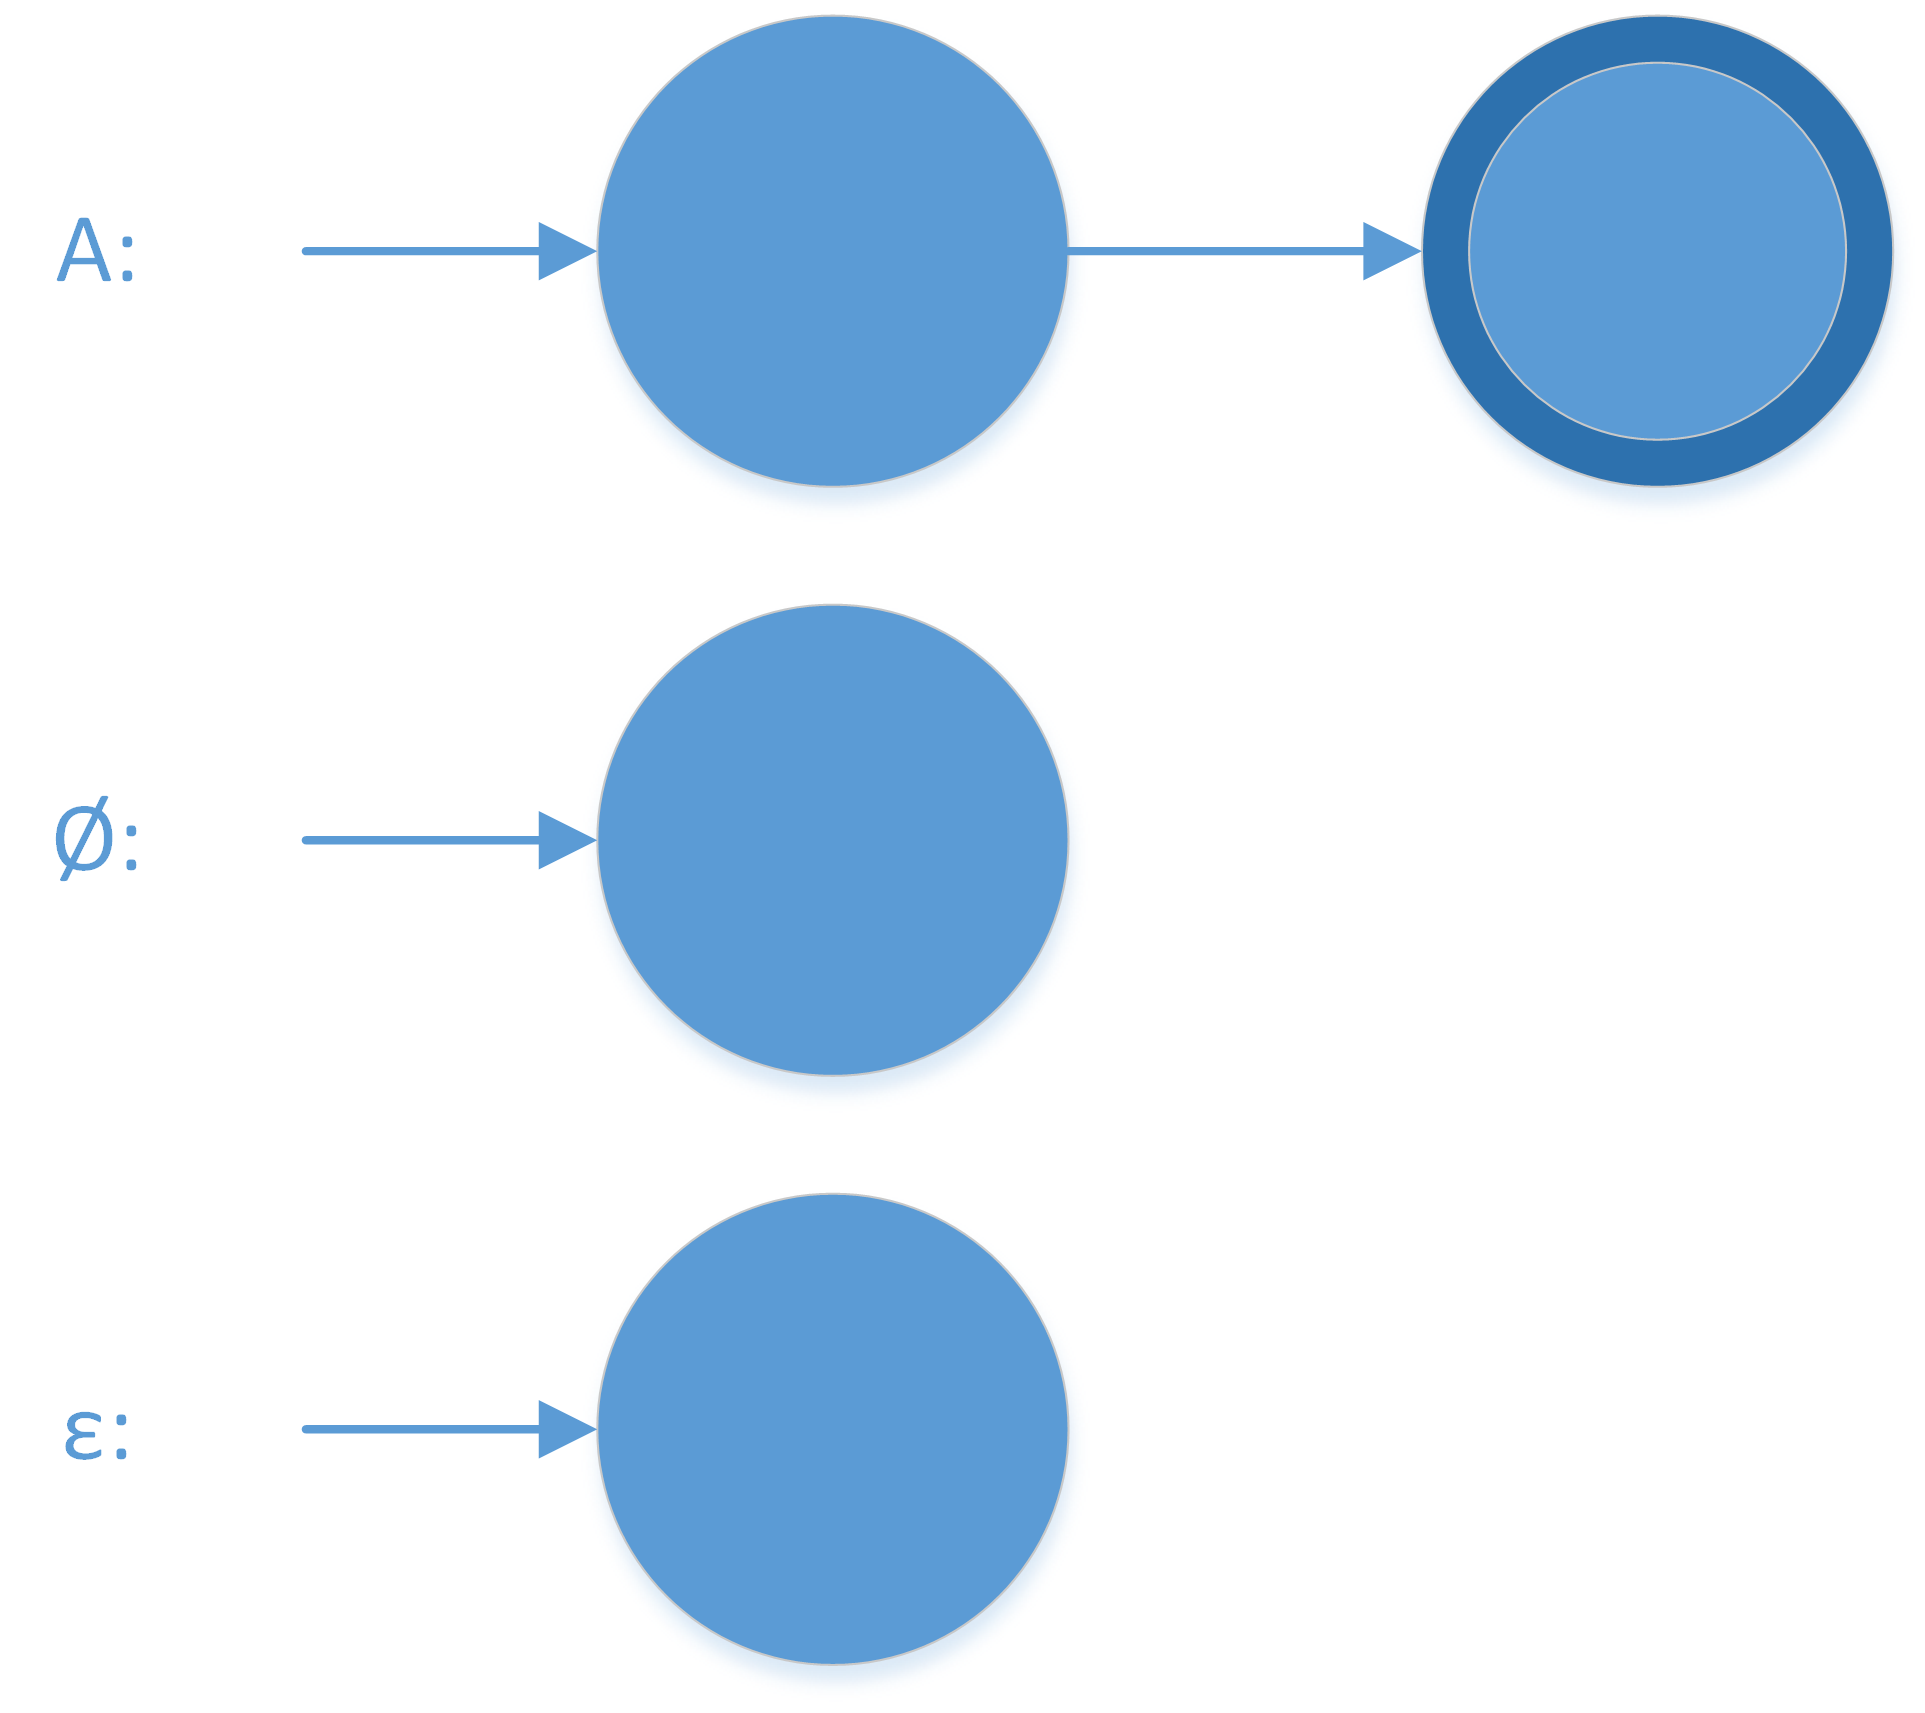
\includegraphics[width=60mm]{Fig1x.png}
\label{fig:fig1}
\caption{Tre tilfælde ved basistrinnet}
\end{figure}

\textbf{Induktionsskrid:}\\
Antag påstand for $K'<K$, hvis for K:


\begin{table}[h]%skal placeres rigtigt
    3 tilfælde:

\begin{tabular}{|l|l|}
        \hline
        $R = (R_1 \cup R_2)$ & Da der findes per induktionsantagelse en $N_1, N_2$ så $L(R_1)=L(N_1)$, $L(R_2)=L(N_2)$. \\
	~ & Vi skal lave en NFA der genkender $L(N_1) \cup L(N_2)$, og det er muligt da de regulære udtryk \\
	~ &  er lukket under $\cup$. \\ 
        $R = (R_1 \circ R_2)$ & Igen findes pr. induktionsantagelse $N_1, N_2$ så $L(R_1) = L(N_1), L(R_2)=L(N_2)$, og det er\\
	~ &  muligt da de regulære sprog er lukket under $\circ$  \\ 
        $(R)^*$ & Pr. induktionsantagelse findes en NFA $N$ så $L(R)=L(N)$. Vi kan lave en NFA som \\
	~&genkender $(L(N))^*$ da de regulære udtryk er lukket under * \\
        \hline
    \end{tabular}
\end{table}

\end{bevis}
\section{Eksempel}
Husk fra tidligere forelæsning konstruktionen af en NFA for $L^*$ (se figur \ref{fig:fig2}) samt $\circ$-konstruktionen (se figur \ref{fig:fig3}).

\begin{figure}[h]%skal placeres rigtigt
\centering
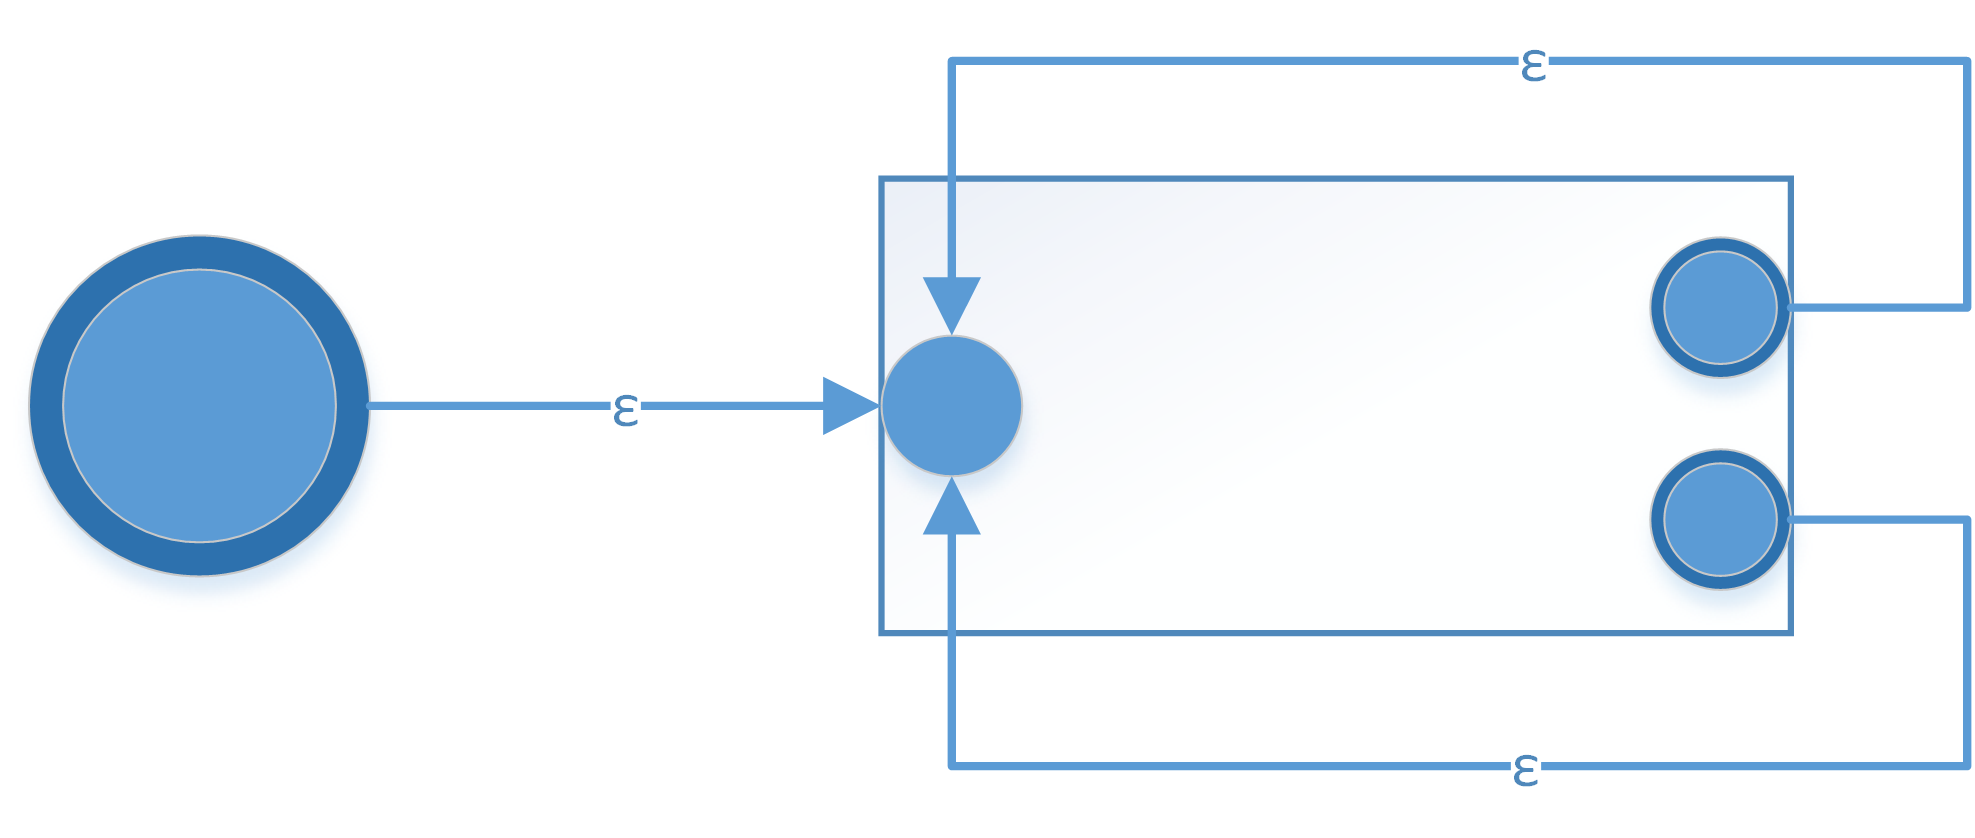
\includegraphics[width=100mm]{Fig2x.png}
\label{fig:fig2}
\caption{*-konstruktion af NFA}
\end{figure}

\begin{figure}[h]%skal placeres rigtigt
\centering
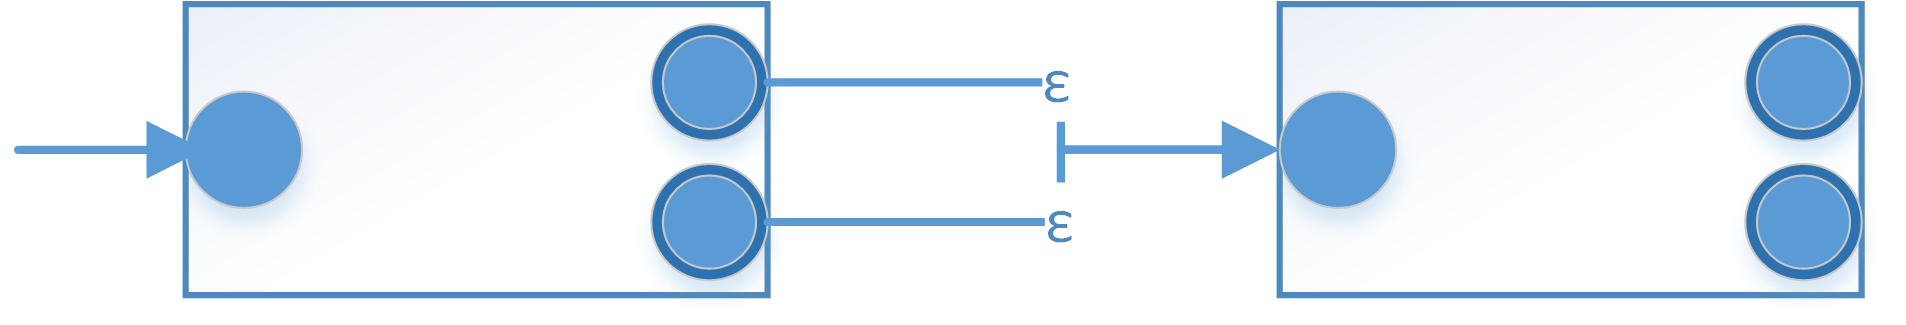
\includegraphics[width=\textwidth]{Fig3x.png}
\label{fig:fig3}
\caption{$\circ$-konstruktionen af NFA}
\end{figure}

Betragt det regulære udtryk $1^*0(1^*01^*01^*)^*  \cup (1 \cup 0)^*11$
For at lave dette regulære udtryk til en NFA starter man inde fra det inderste led, og arbejder sig ud. I dette tilfælde starter man altså med at konstruere en NFA for 0 og 1, som set på figur \ref{fig:fig4}.

\begin{figure}[h]%skal placeres rigtigt
\centering
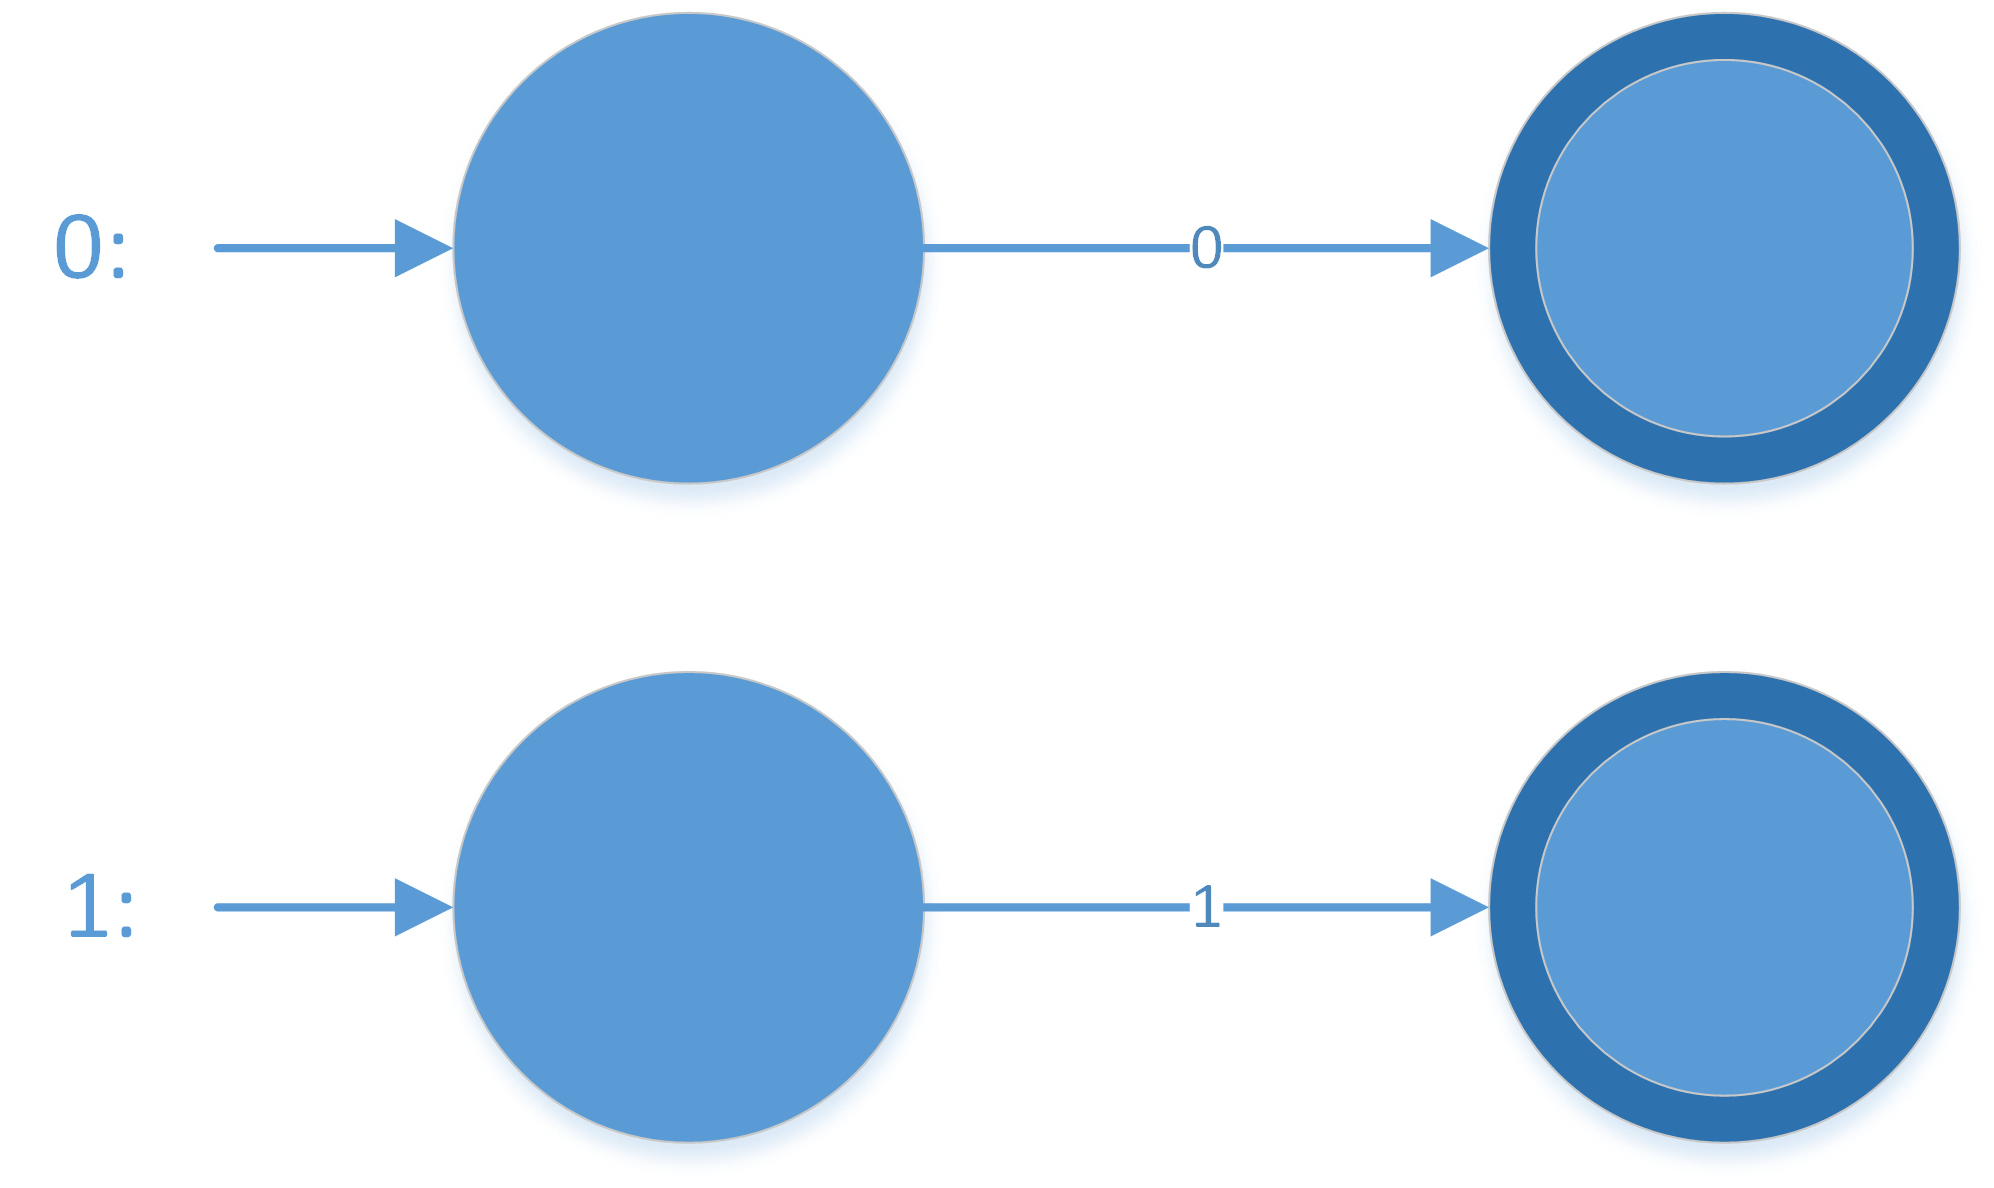
\includegraphics[width=\textwidth]{Fig4x.png}
\label{fig:fig4}
\caption{NFA for 1 og 0}
\end{figure}

Herefter konstrueres NFA'en for $1^*$ som set på figur \ref{fig:fig5}. 

\begin{figure}[h]%skal placeres rigtigt
\centering
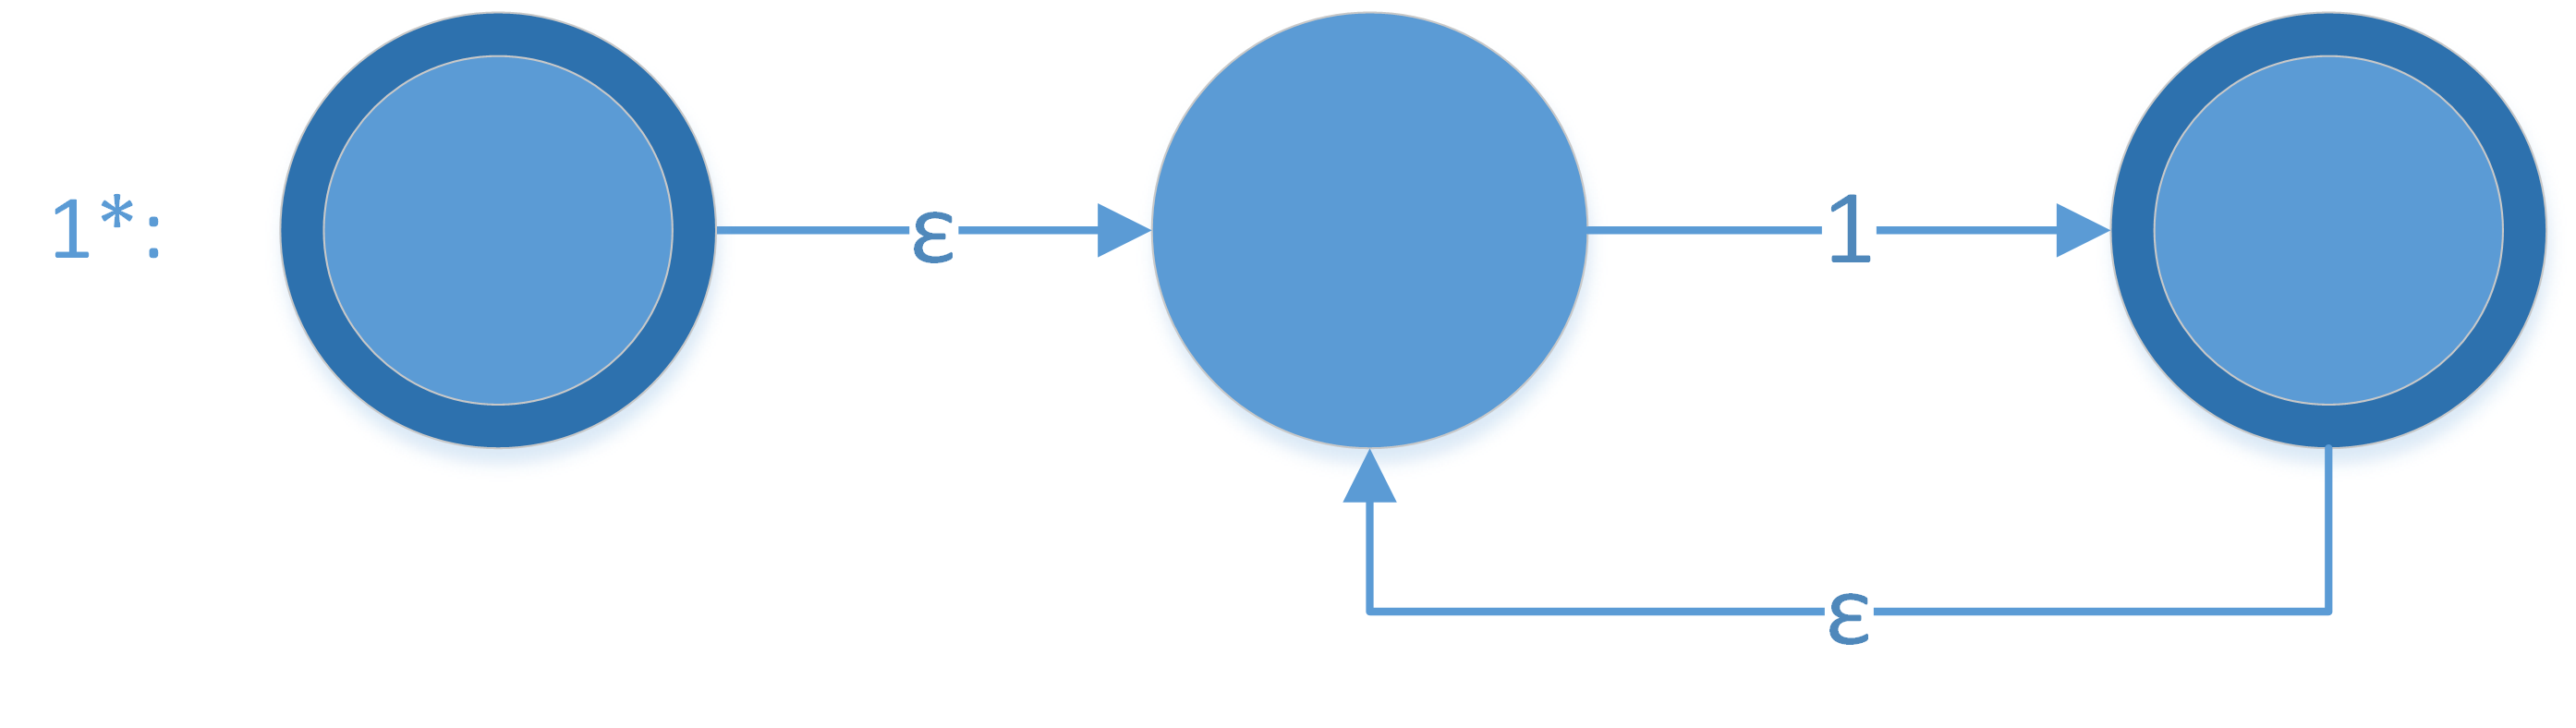
\includegraphics[width=\textwidth]{Fig5x.png}
\label{fig:fig5}
\caption{NFA for $1^*$}
\end{figure}

Herefter konstrueres NFA'en for $1^*0$ som set på figur \ref{fig:fig6}. 

\begin{figure}[h]%skal placeres rigtigt
\centering
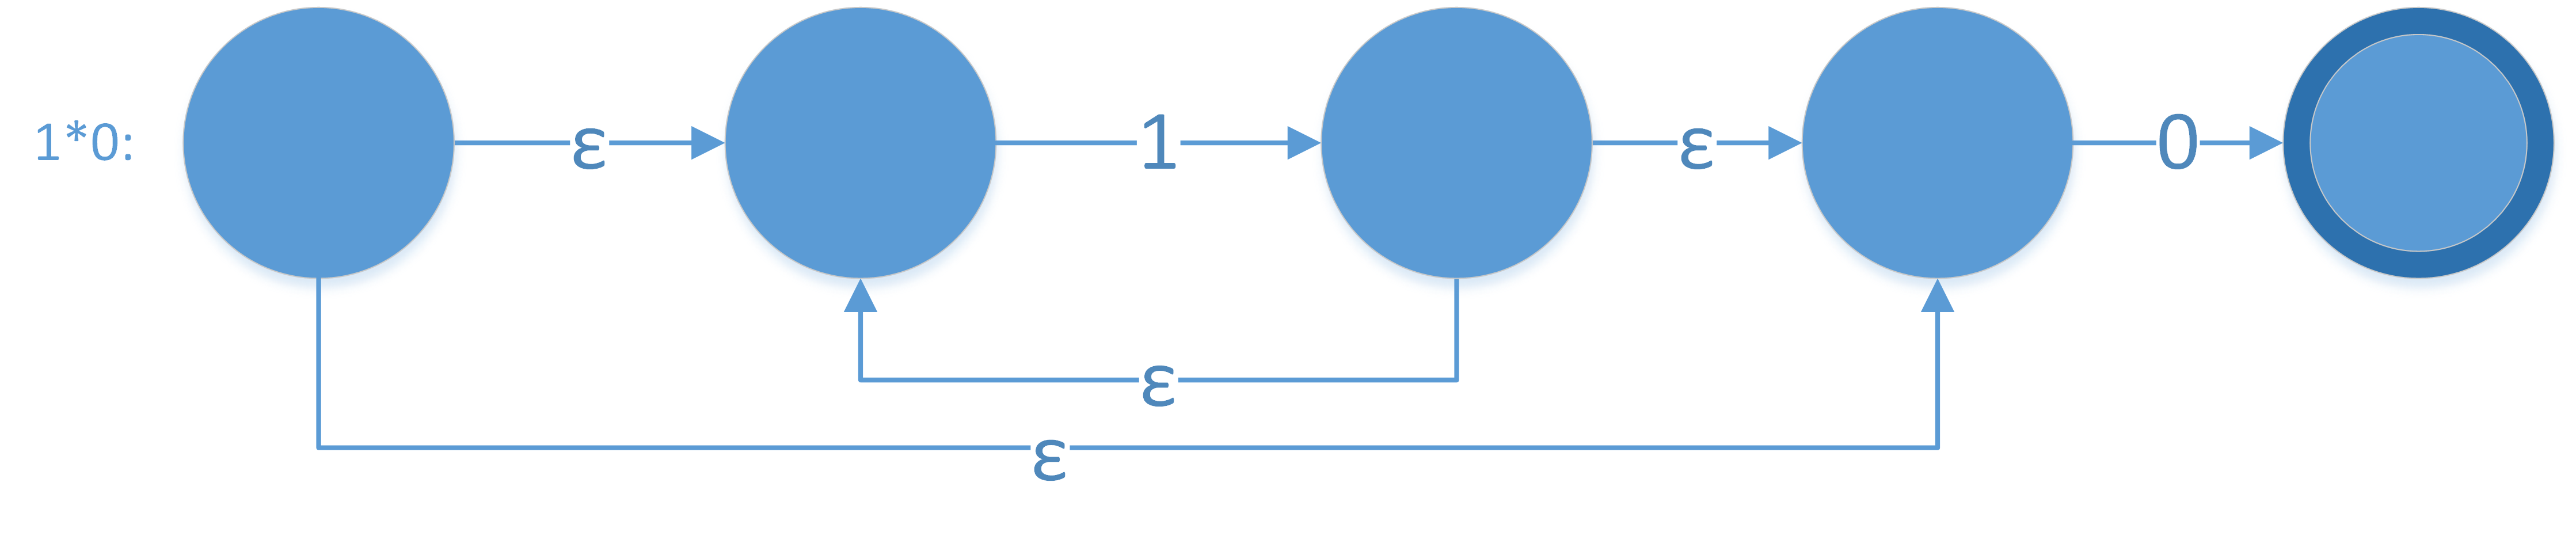
\includegraphics[width=\textwidth]{Fig6x.png}
\label{fig:fig6}
\caption{NFA for $1^*0$}
\end{figure}

Herefter konstrueres NFA'en for $1^*01^*0$ som set på figur \ref{fig:fig7}. 

\begin{figure}[h]%skal placeres rigtigt
\centering
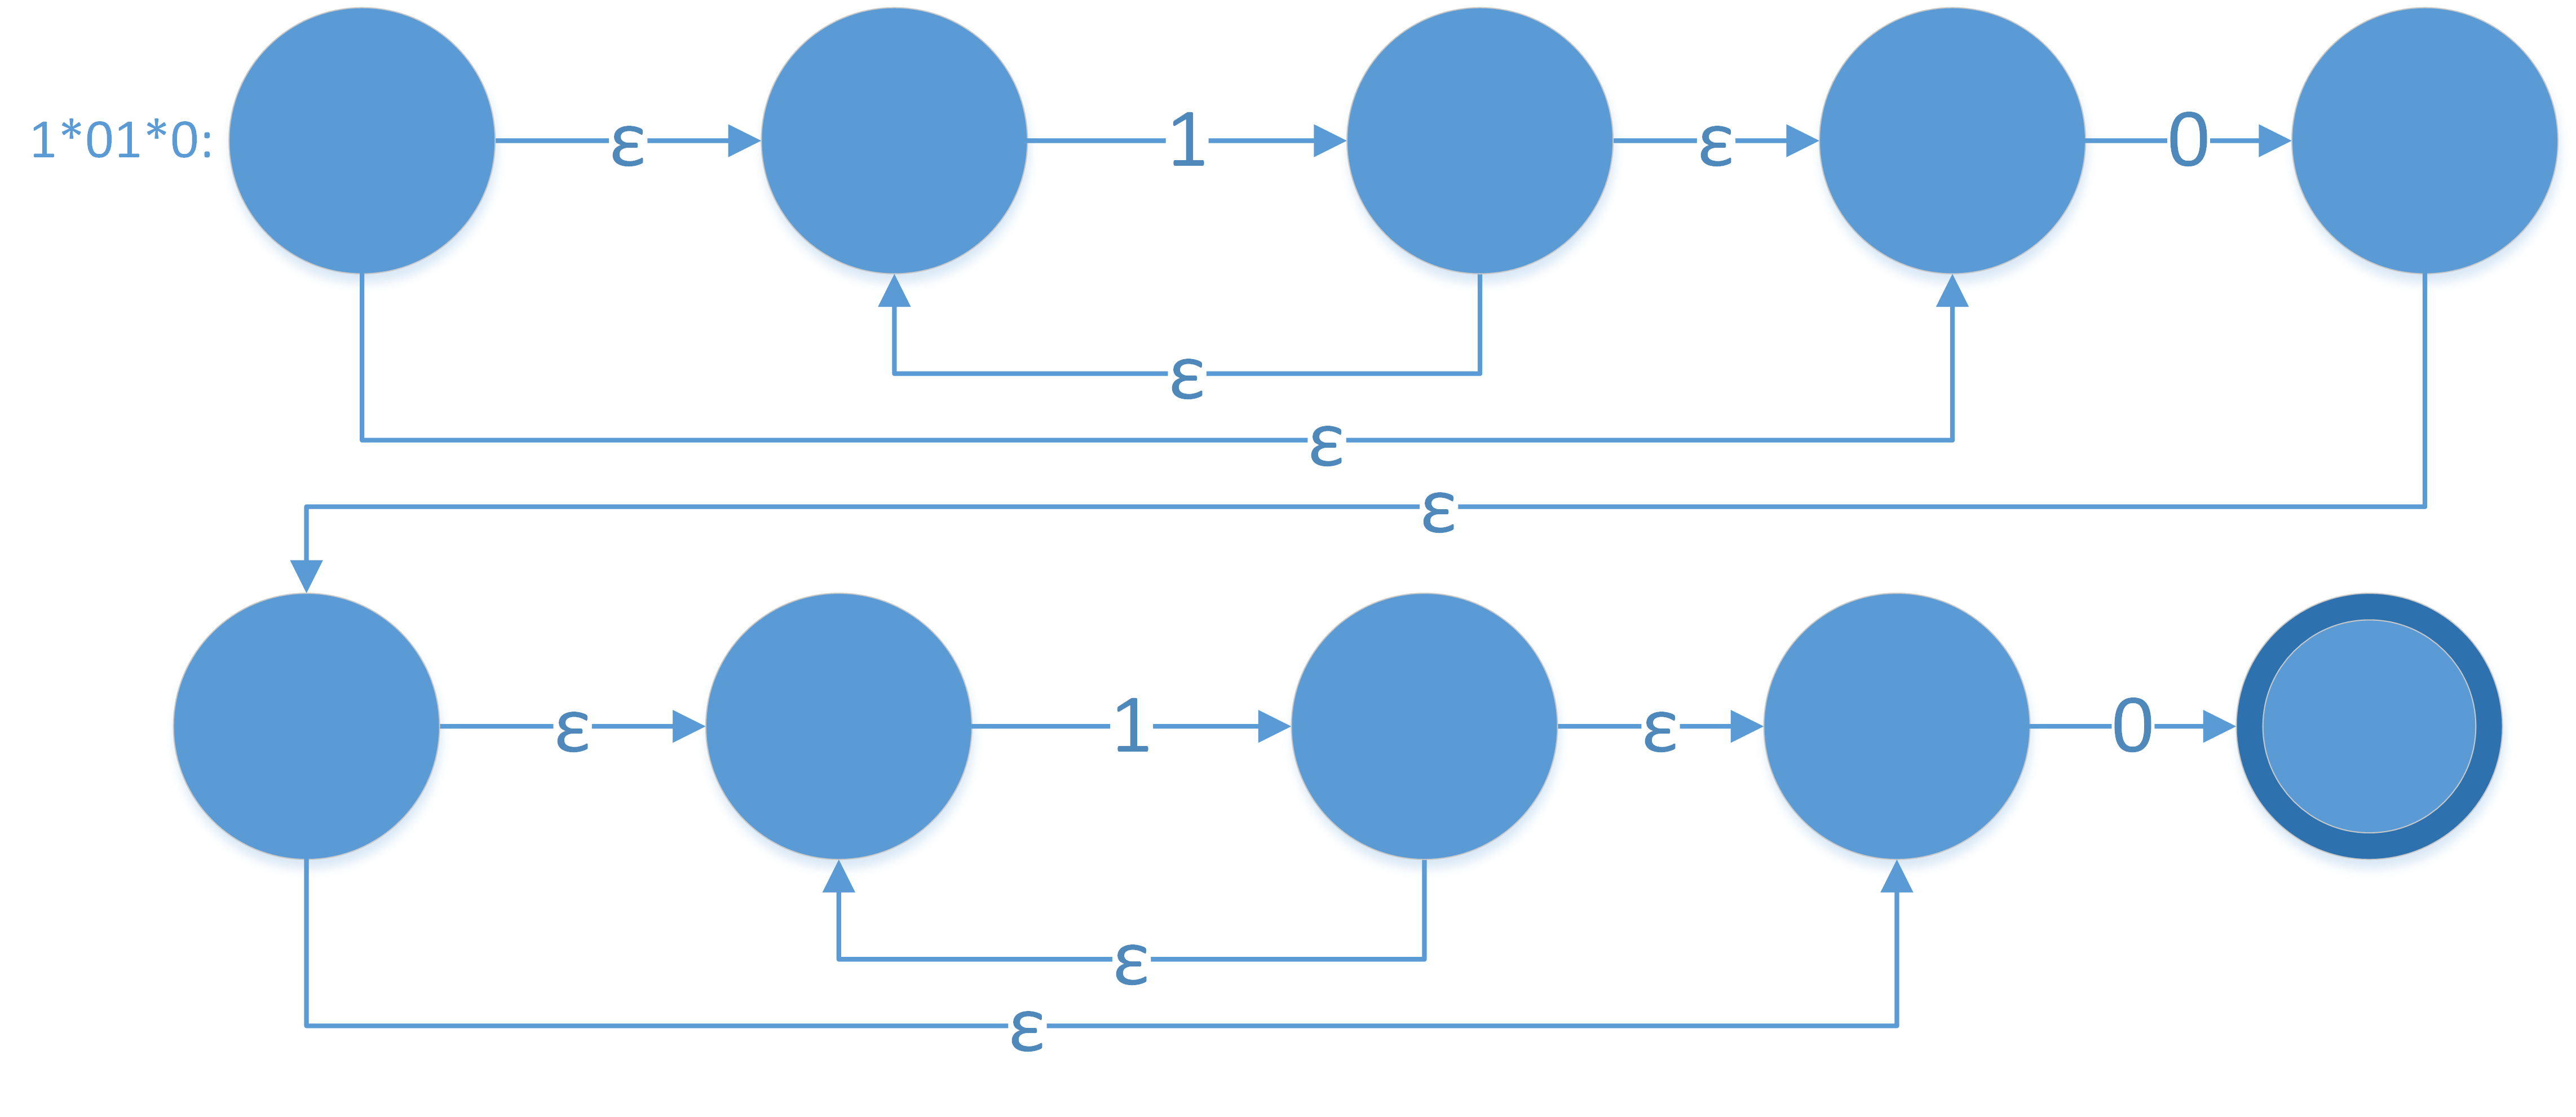
\includegraphics[width=\textwidth]{Fig7x.png}
\label{fig:fig7}
\caption{NFA for $1^*01^*0$}
\end{figure}

Herefter konstrueres NFA'en for $1^*01^*01^*$ som set på figur \ref{fig:fig8}. 

\begin{figure}[h]%skal placeres rigtigt
\centering
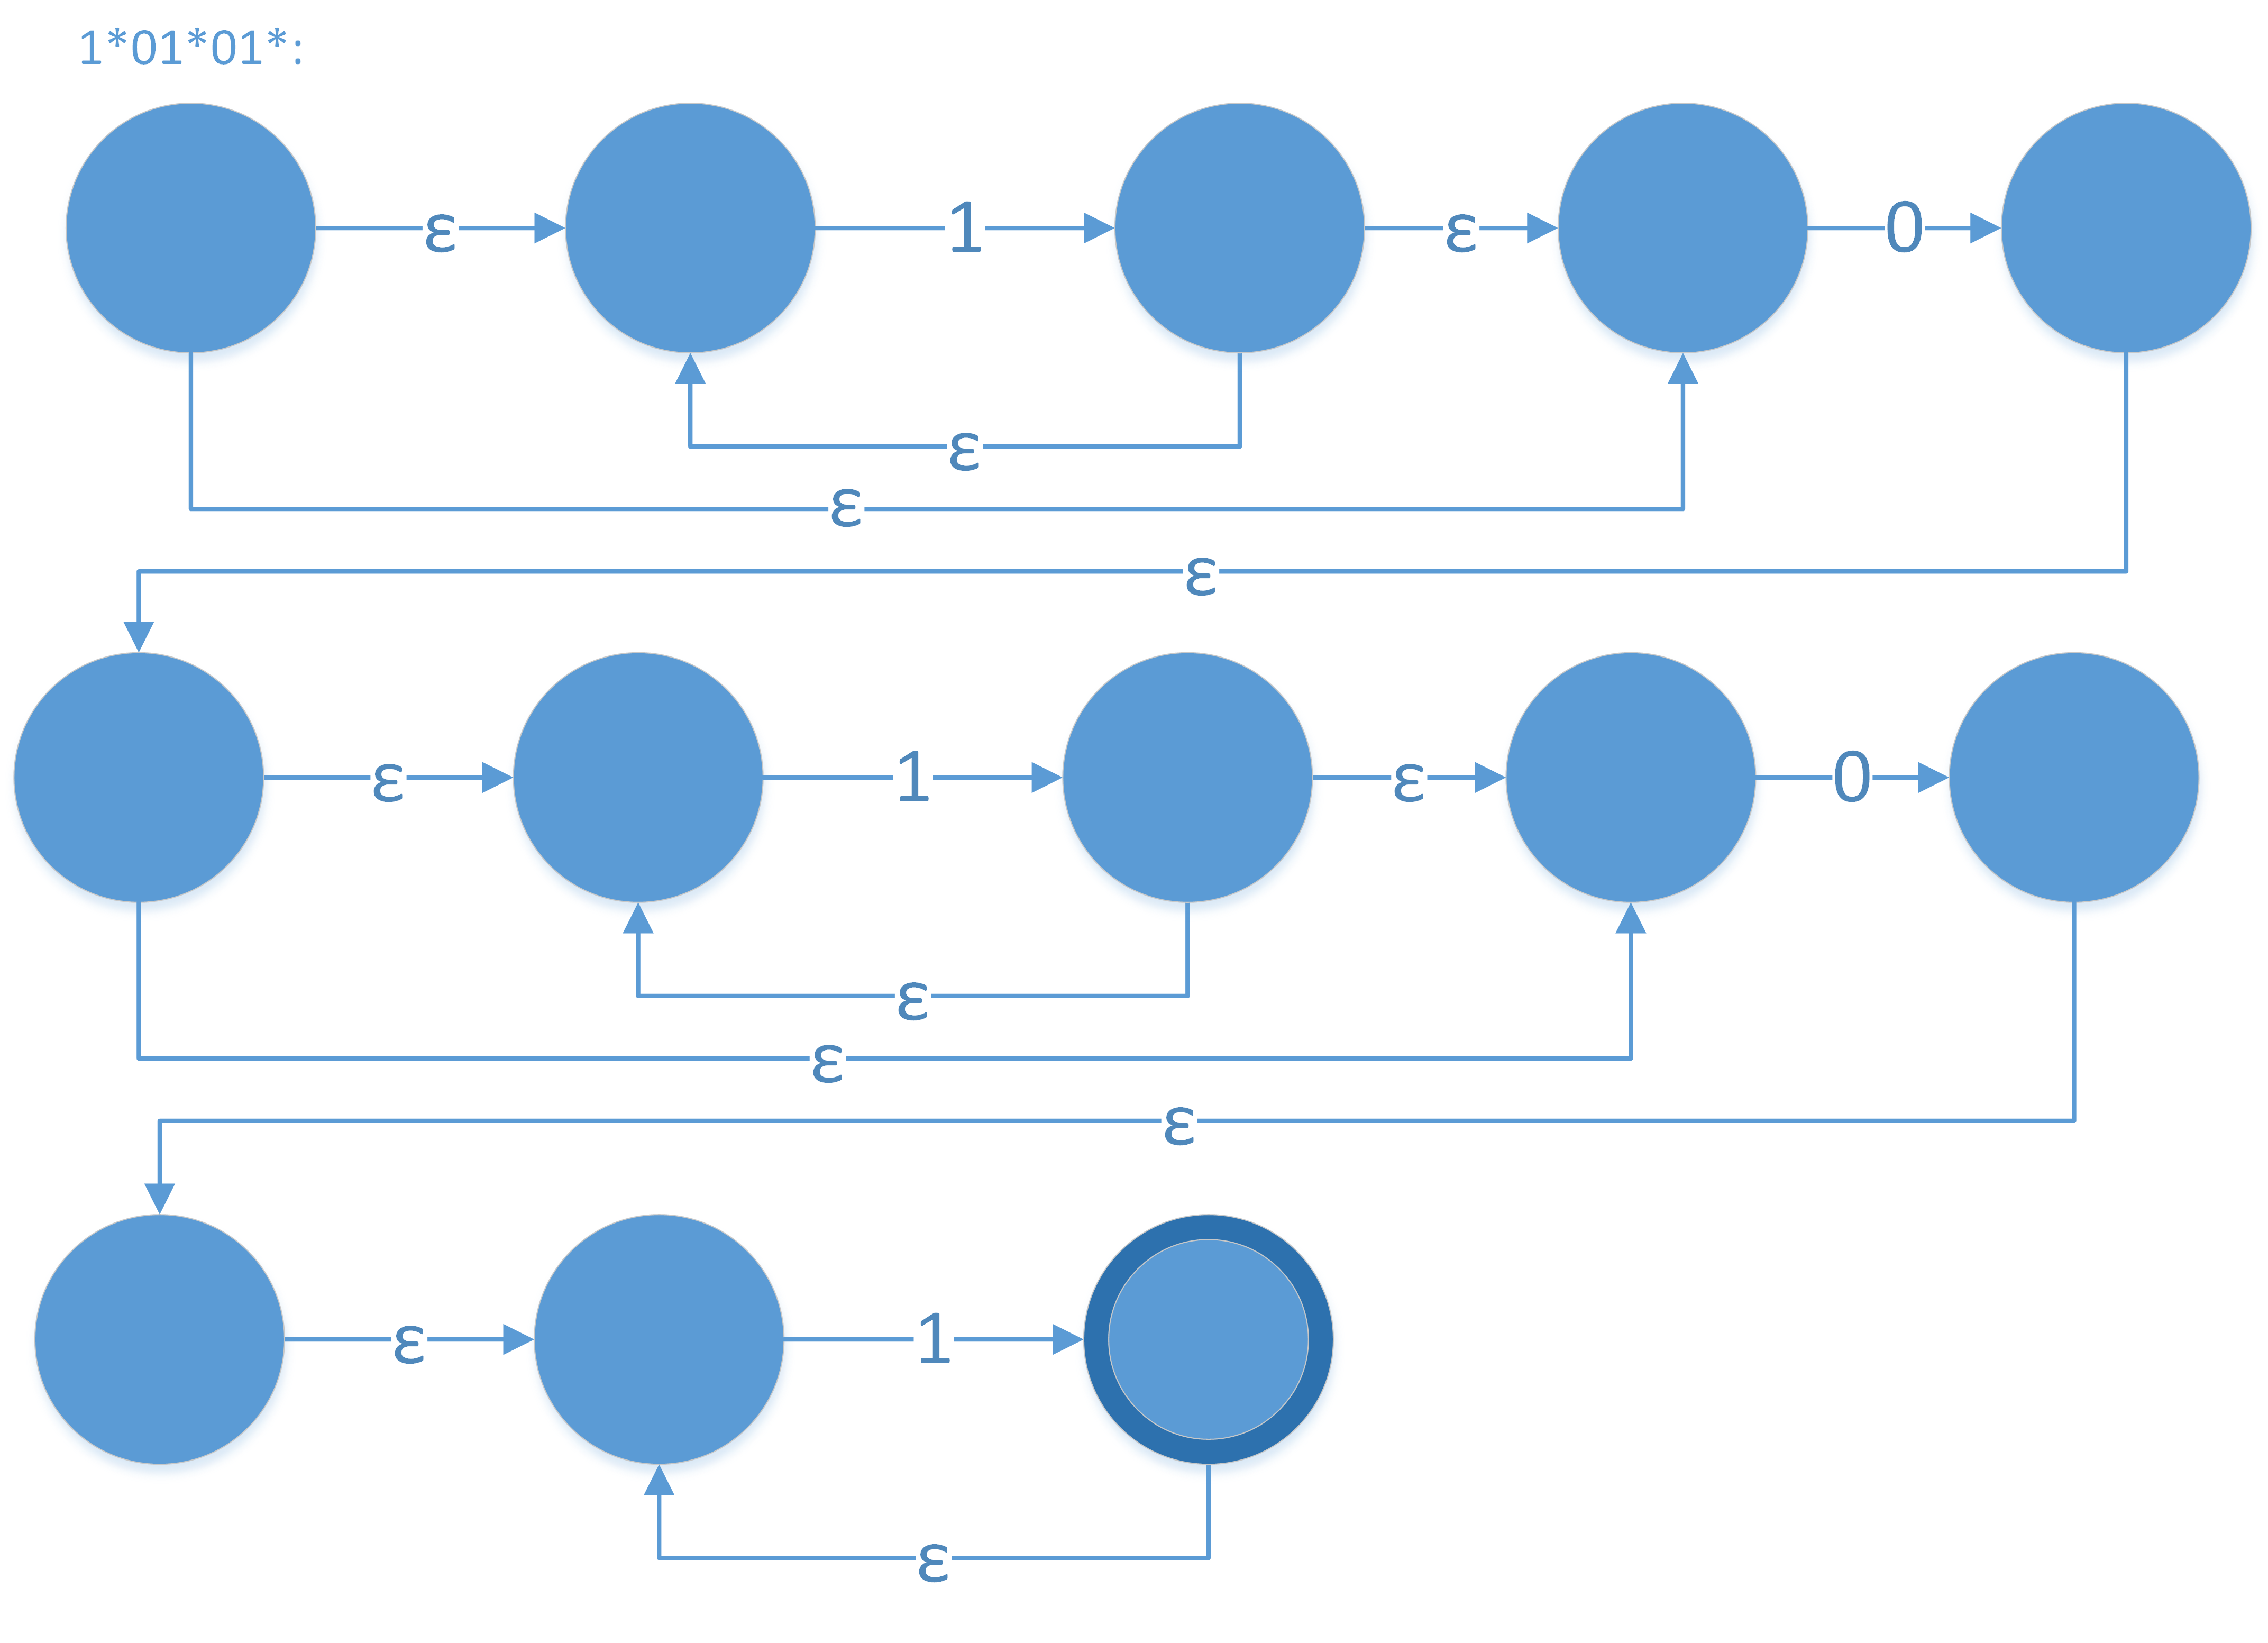
\includegraphics[width=\textwidth]{Fig8x.png}
\label{fig:fig8}
\caption{NFA for $1^*01^*01^*$}
\end{figure}

Herefter konstrueres NFA'en for $(1^*01^*01^*)^*$ som set på figur \ref{fig:fig9}. Denne NFA kaldes fremover N.

\begin{figure}[h]%skal placeres rigtigt
\centering
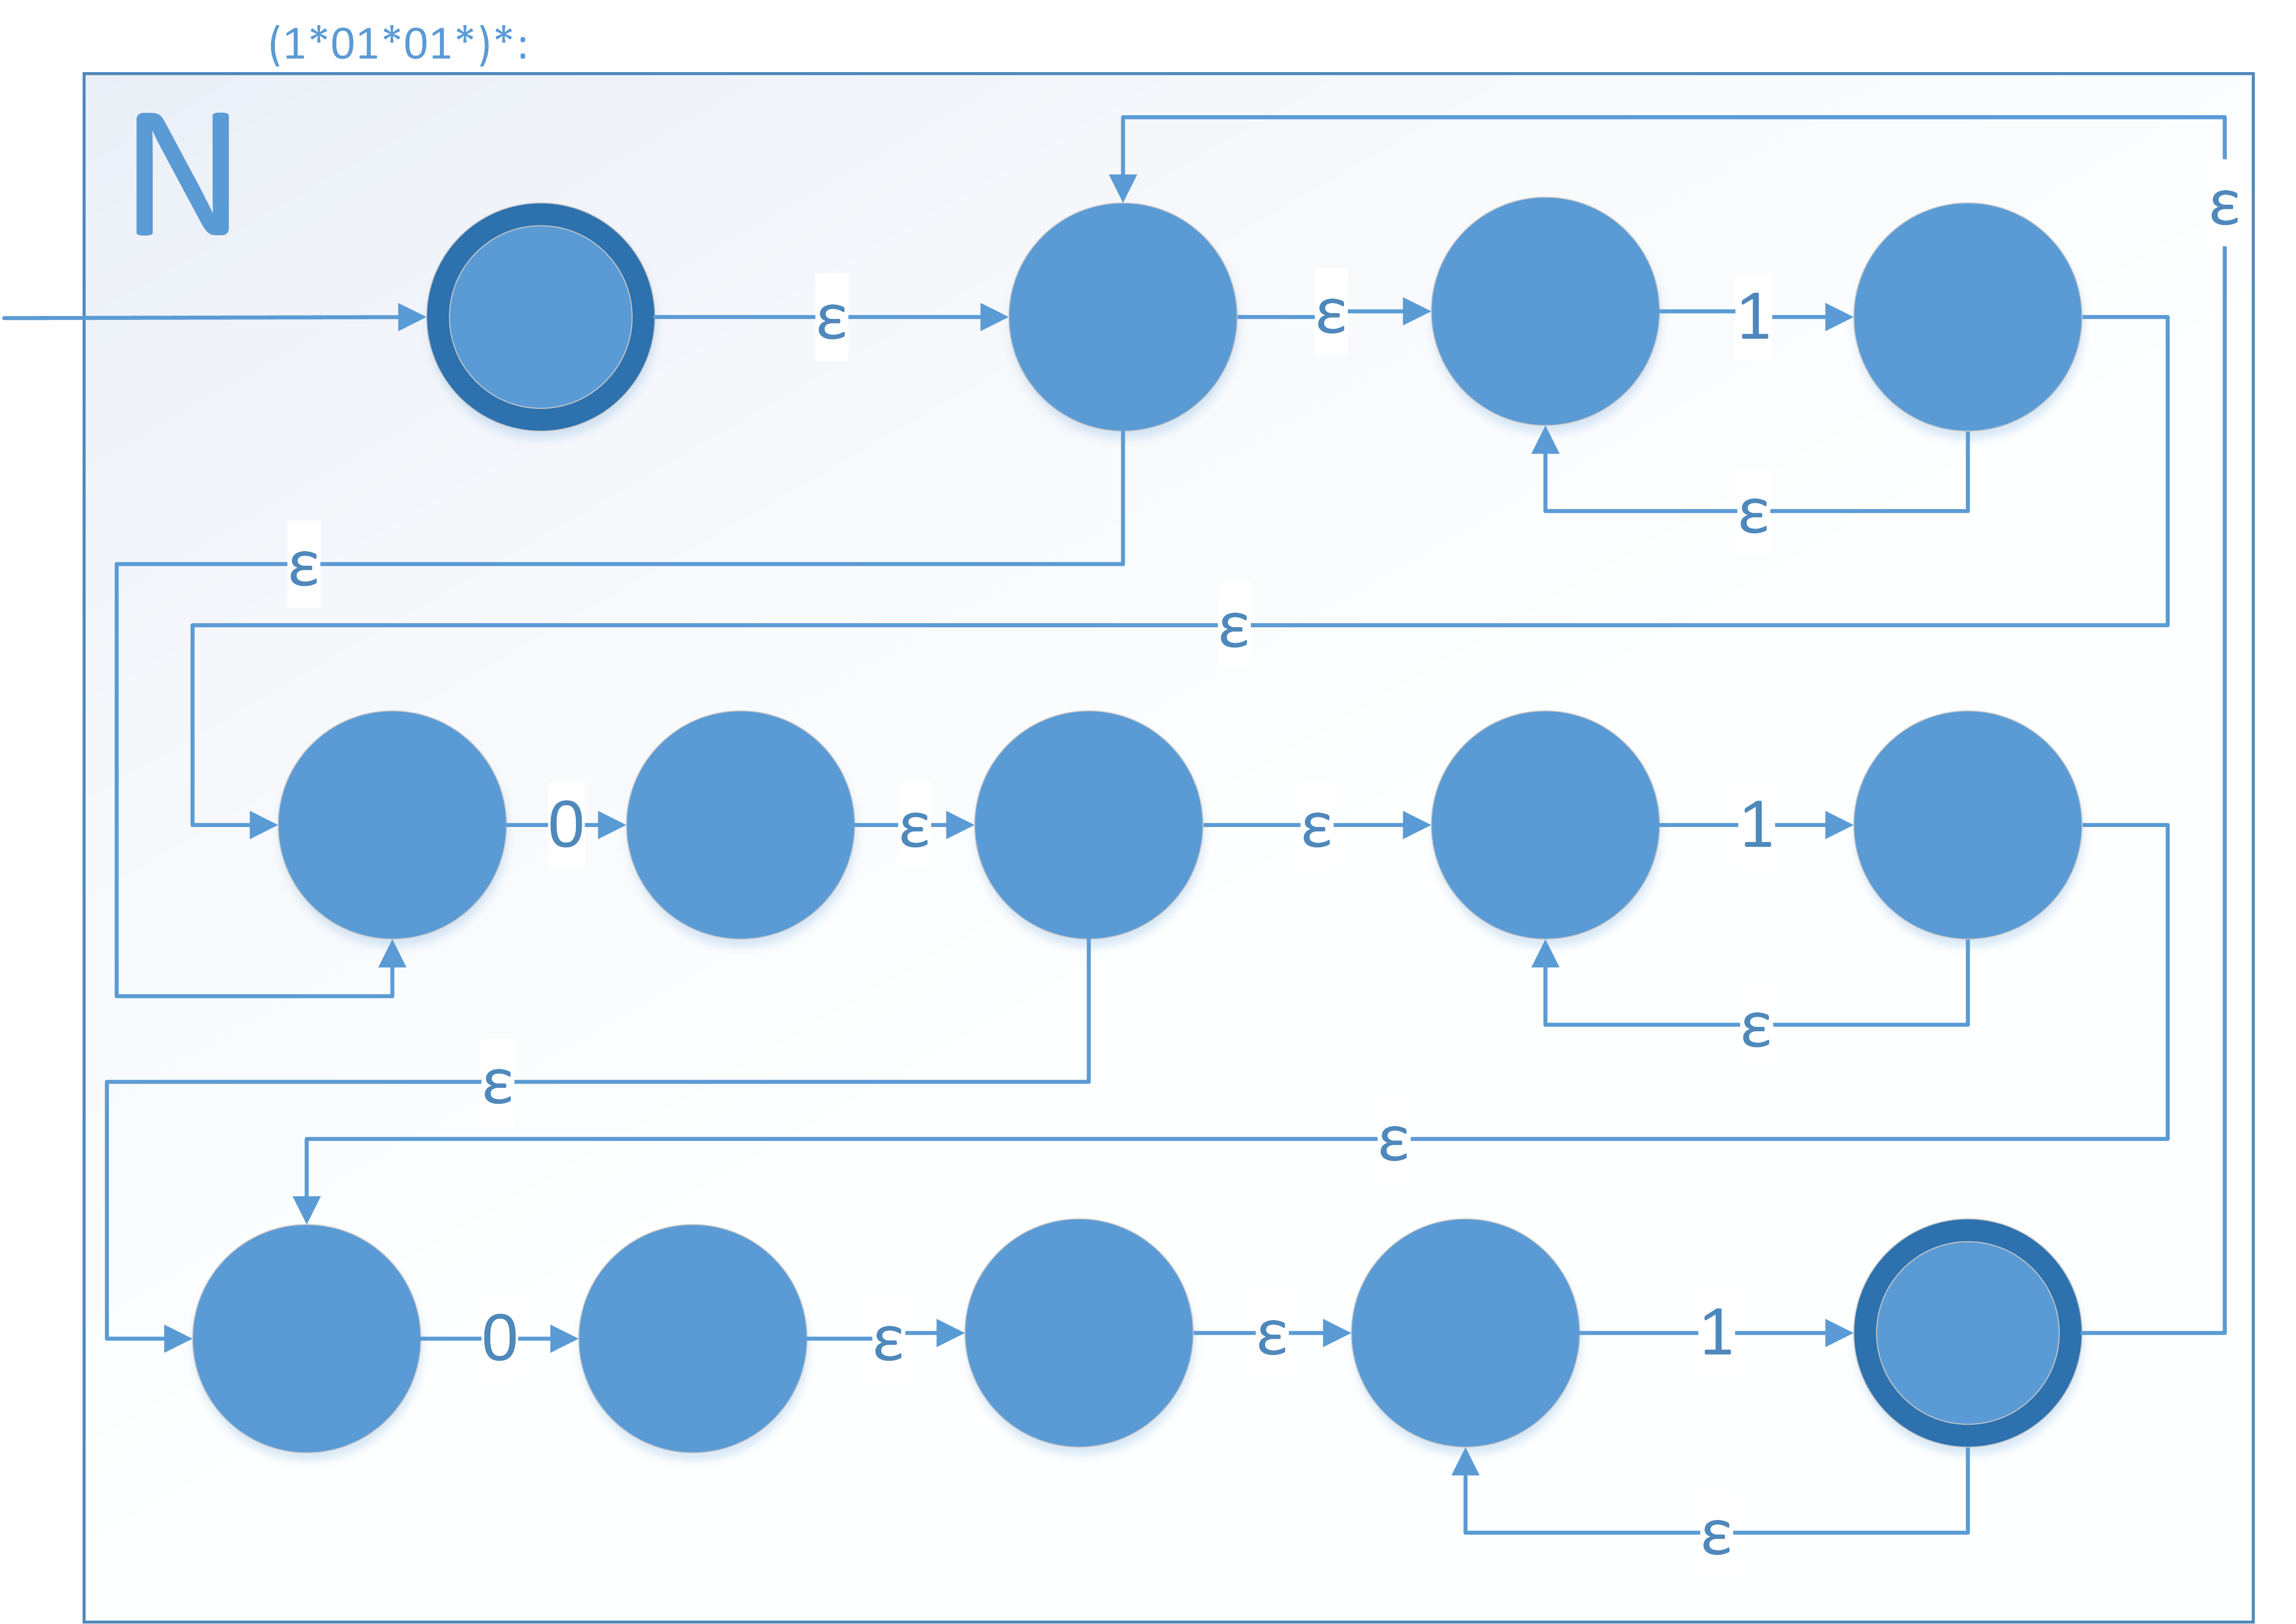
\includegraphics[width=\textwidth]{Fig9x.png}
\label{fig:fig9}
\caption{NFA for $(1^*01^*01^*)^*$}
\end{figure}

Herefter konstrueres NFA'en for $1*0(1^*01^*01^*)^*$ som set på figur \ref{fig:fig10}. Denne NFA kaldes fremover N'.

\begin{figure}[h]%skal placeres rigtigt
\centering
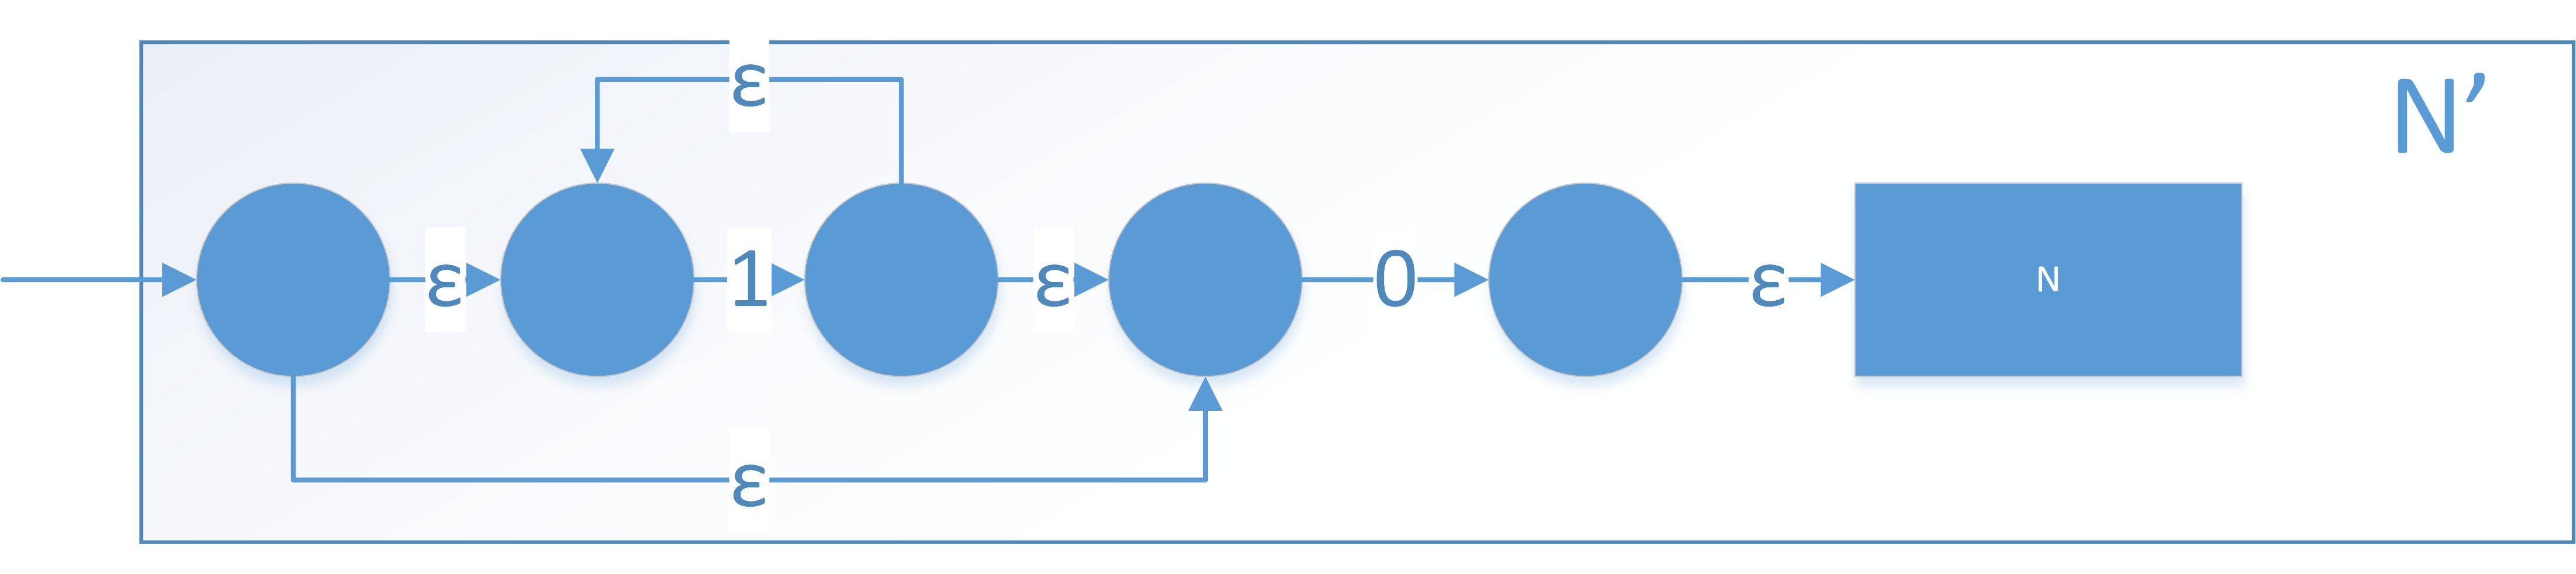
\includegraphics[width=\textwidth]{Fig10x.png}
\label{fig:fig10}
\caption{NFA for $1^*0(1^*01^*01^*)^*$}
\end{figure}

Herefter konstrueres NFA'en for $0\cup1$ som set på figur \ref{fig:fig11}.

\begin{figure}[h]%skal placeres rigtigt
\centering
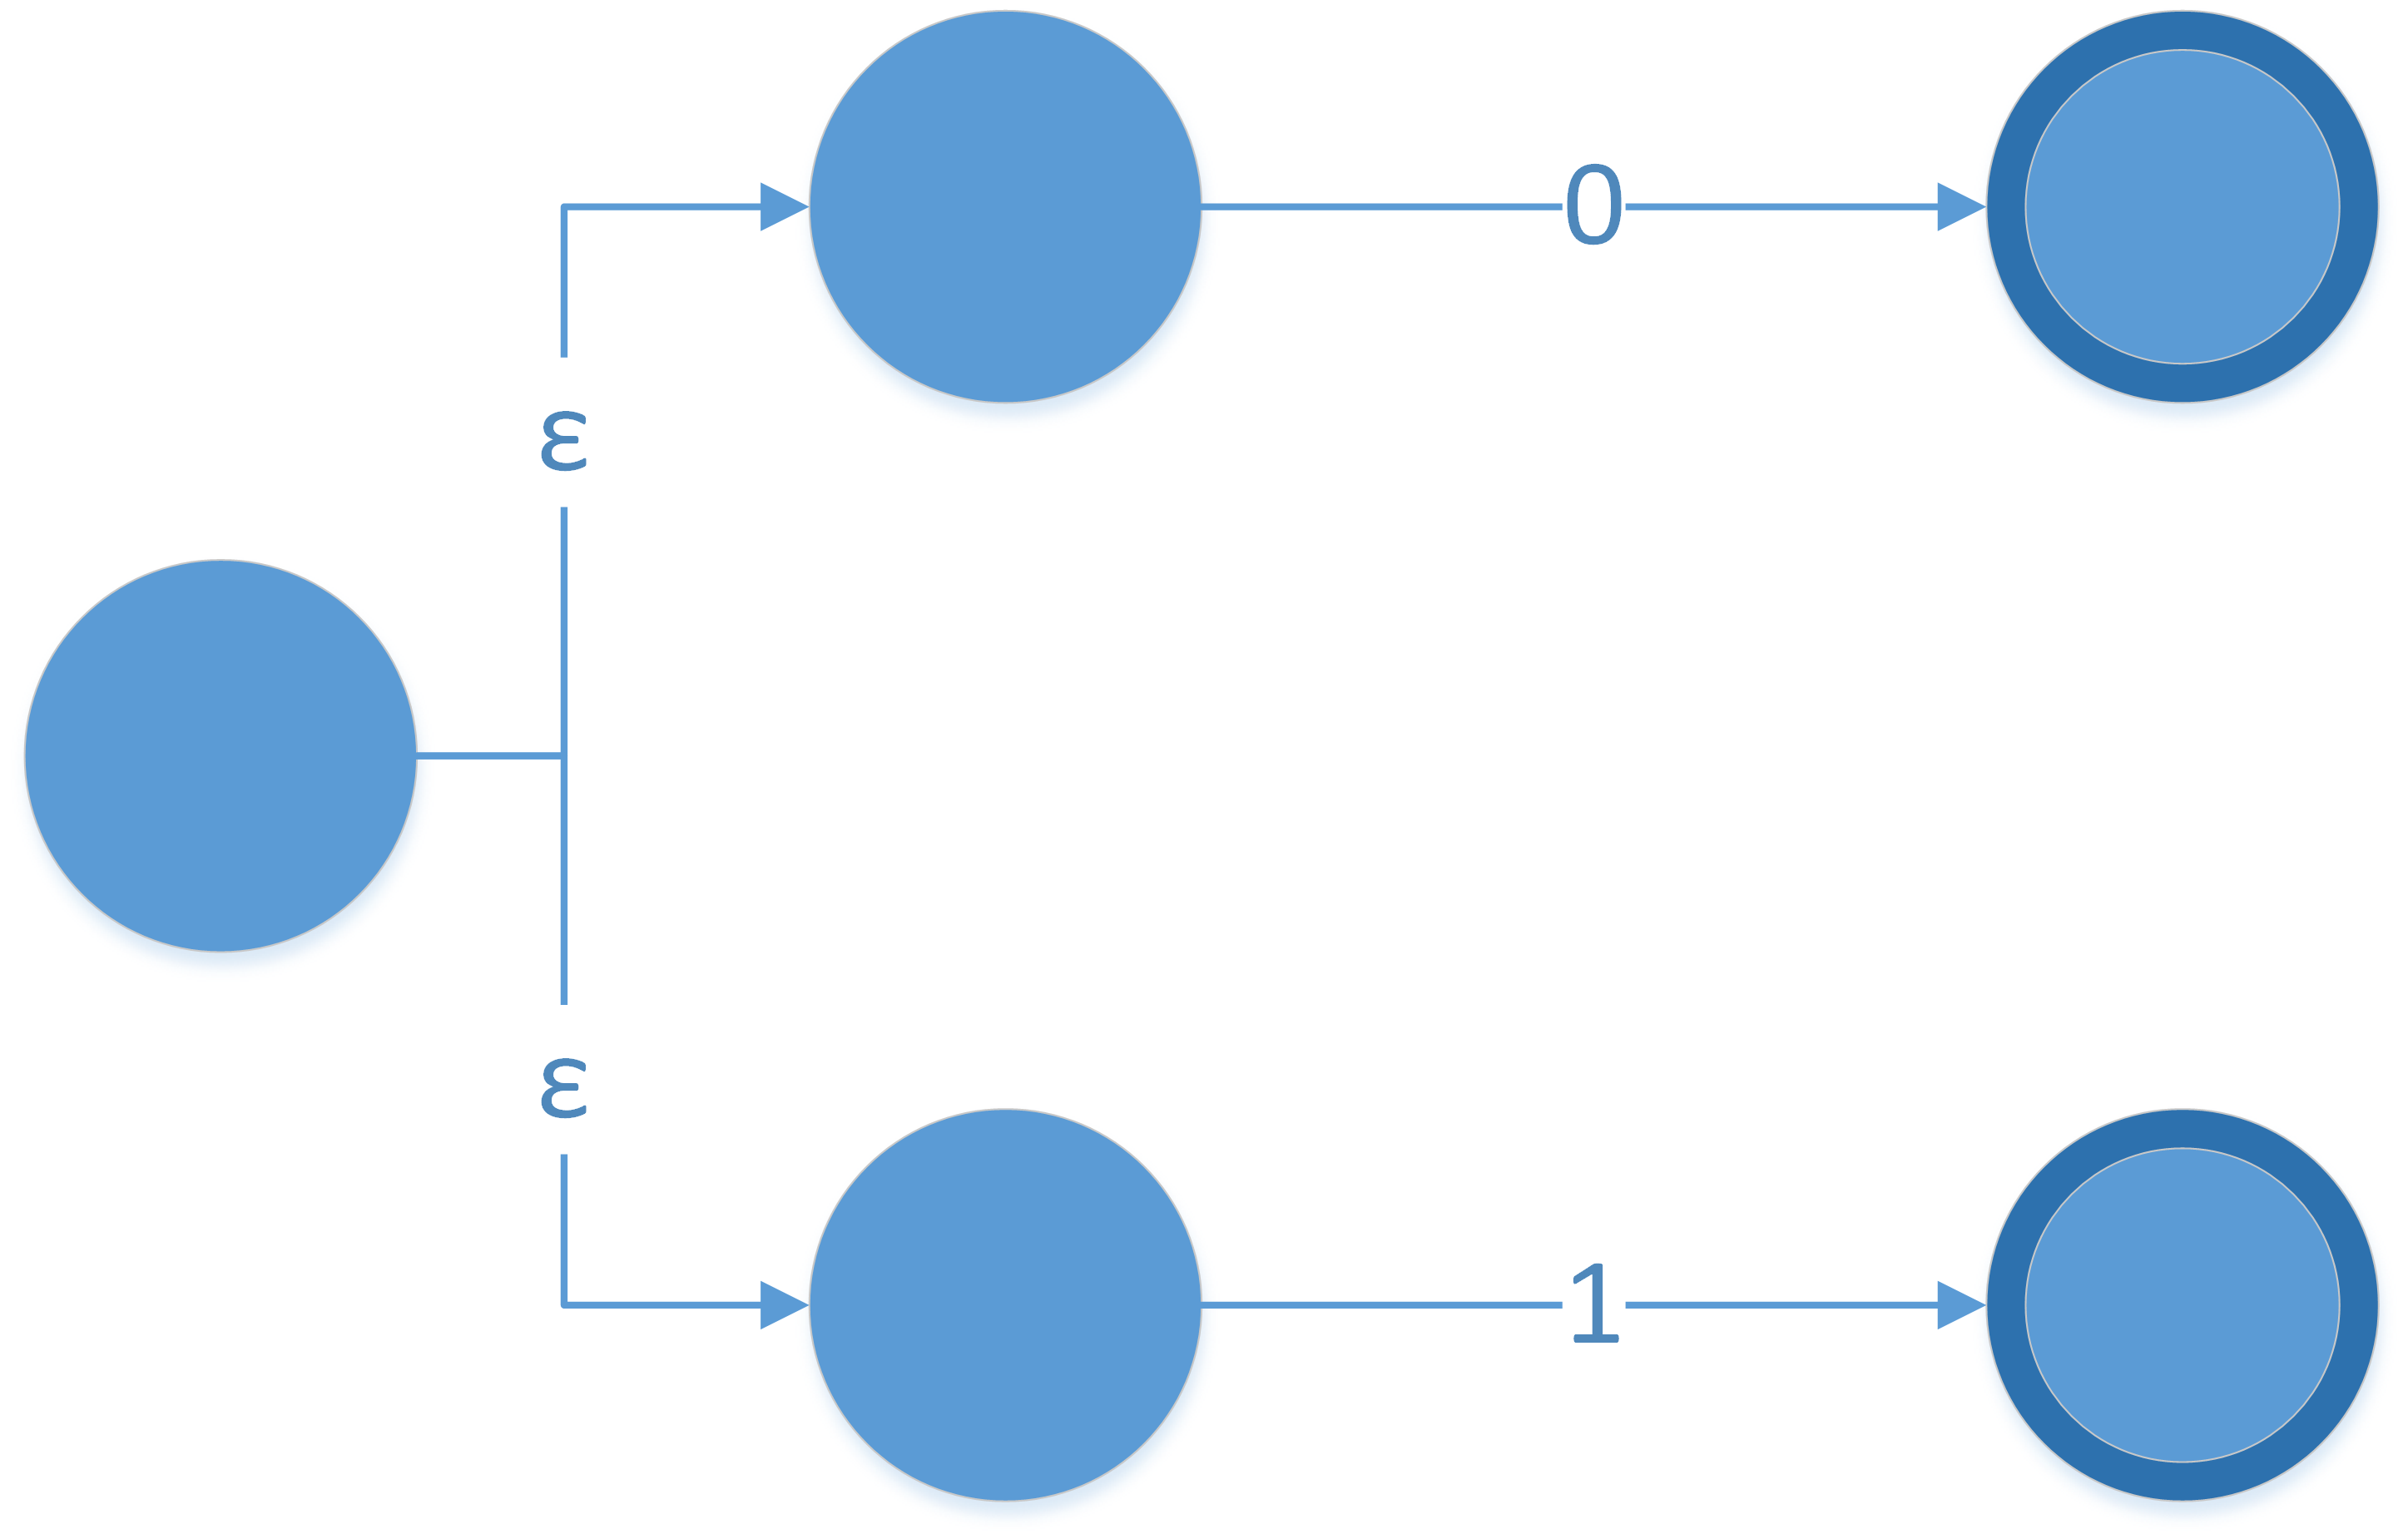
\includegraphics[width=\textwidth]{Fig11x.png}
\label{fig:fig11}
\caption{NFA for $0\cup1$}
\end{figure}
Herefter konstrueres NFA'en for $(0\cup1)^*$ som set på figur \ref{fig:fig12}.

\begin{figure}[h]%skal placeres rigtigt
\centering
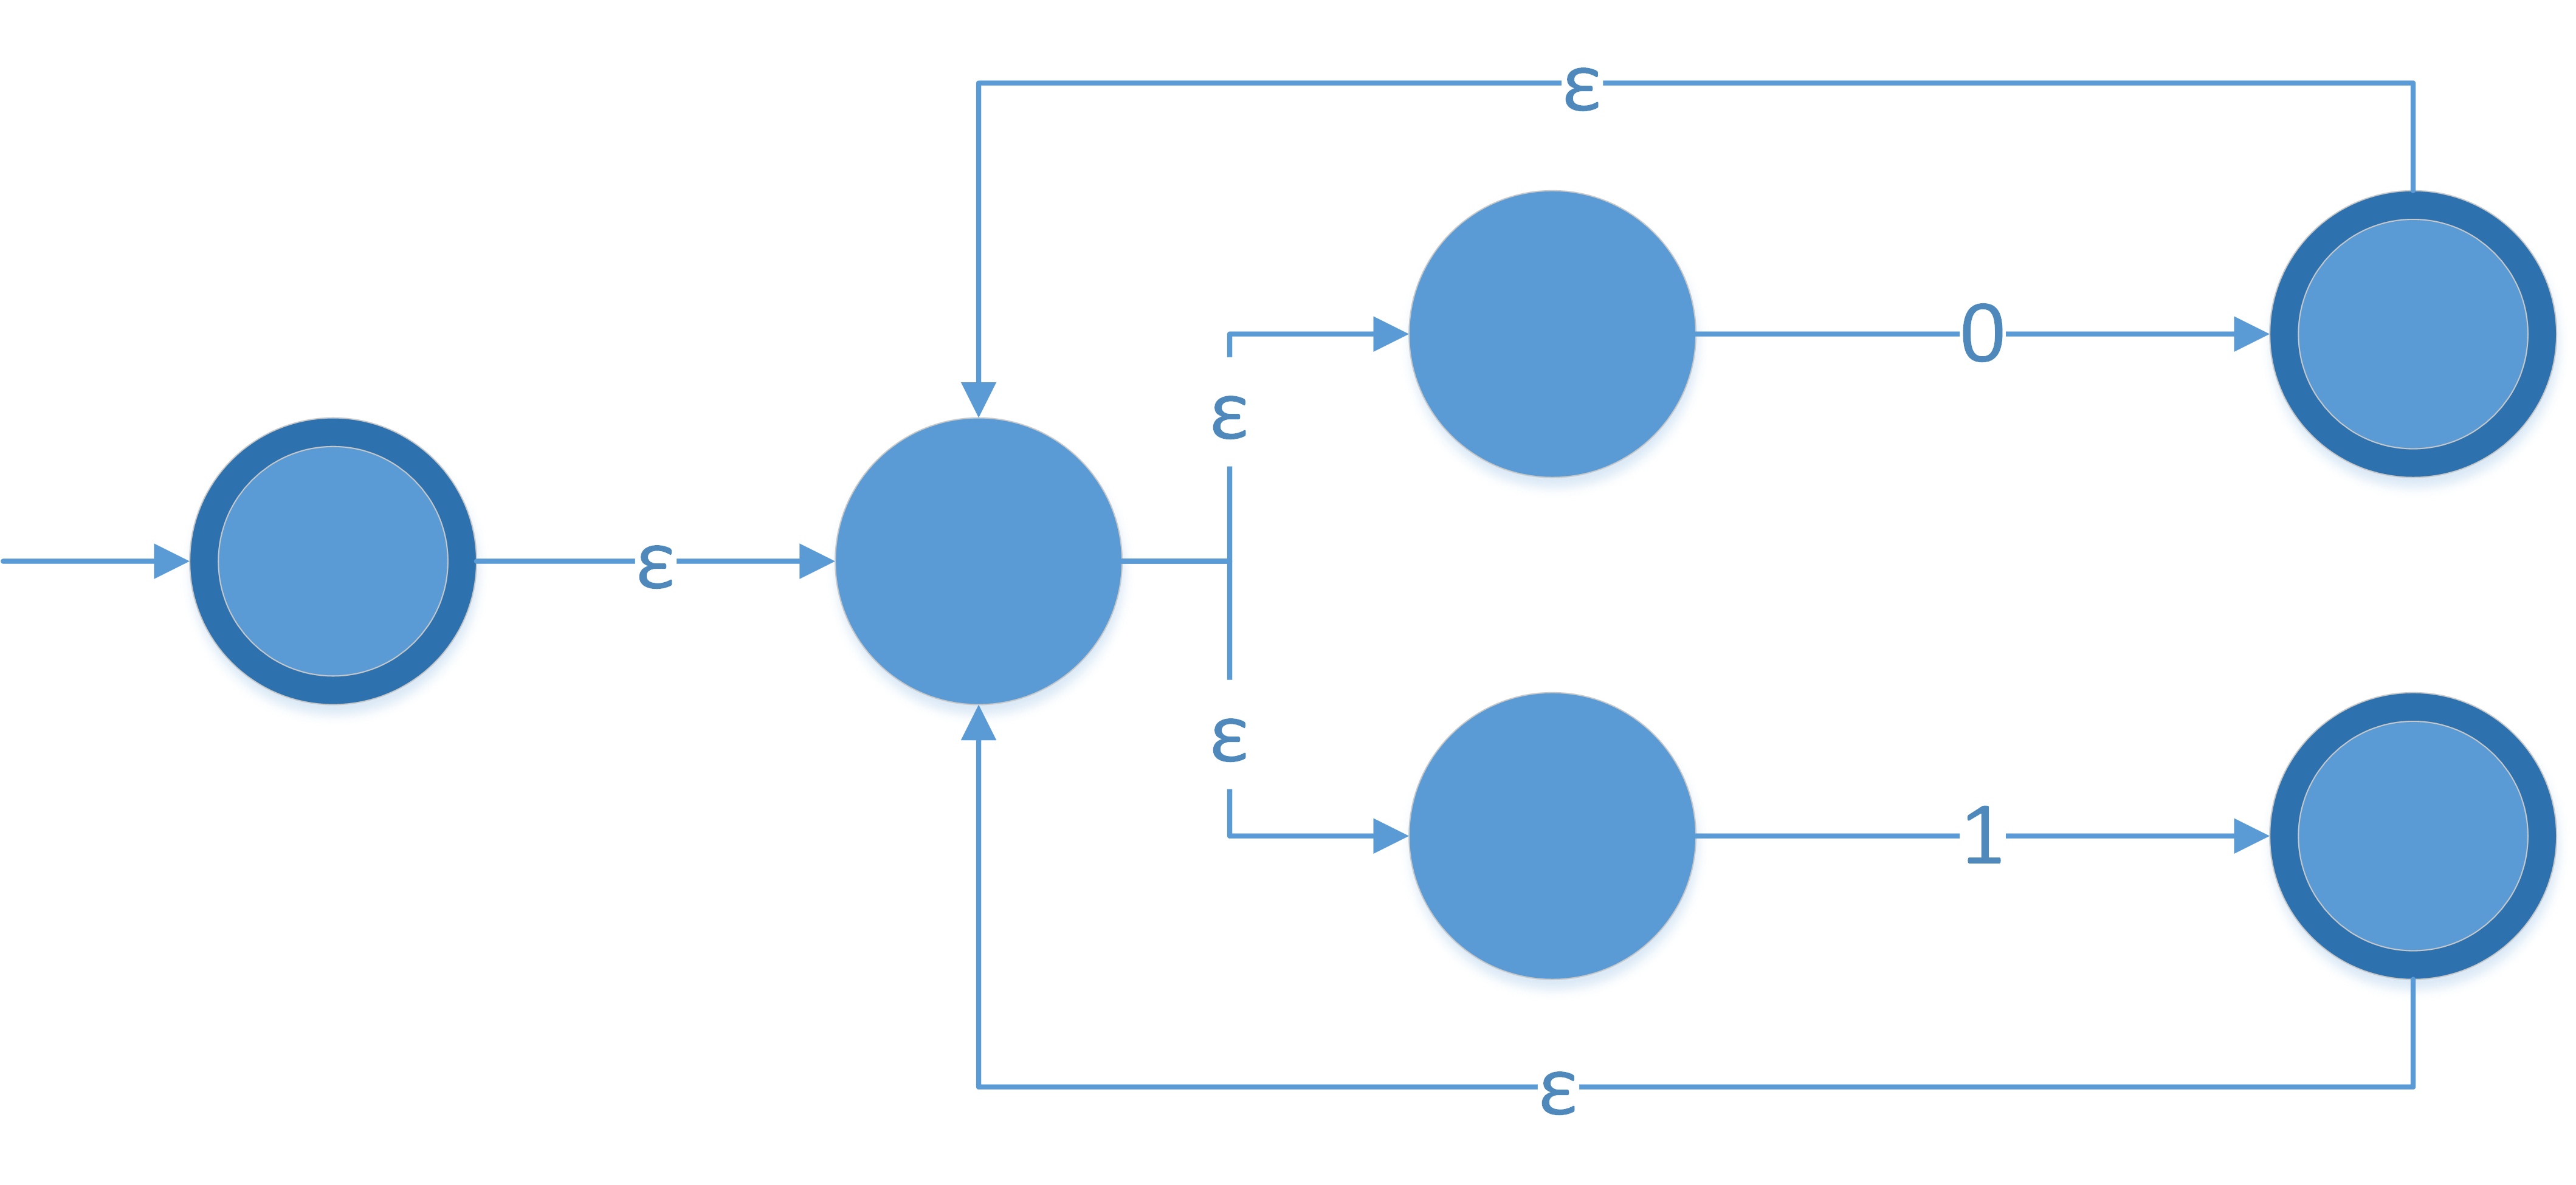
\includegraphics[width=\textwidth]{Fig12x.png}
\label{fig:fig12}
\caption{NFA for $(0\cup1)^*$}
\end{figure}

Herefter konstrueres NFA'en for $11$ som set på figur \ref{fig:fig13}.

\begin{figure}[h]%skal placeres rigtigt
\centering
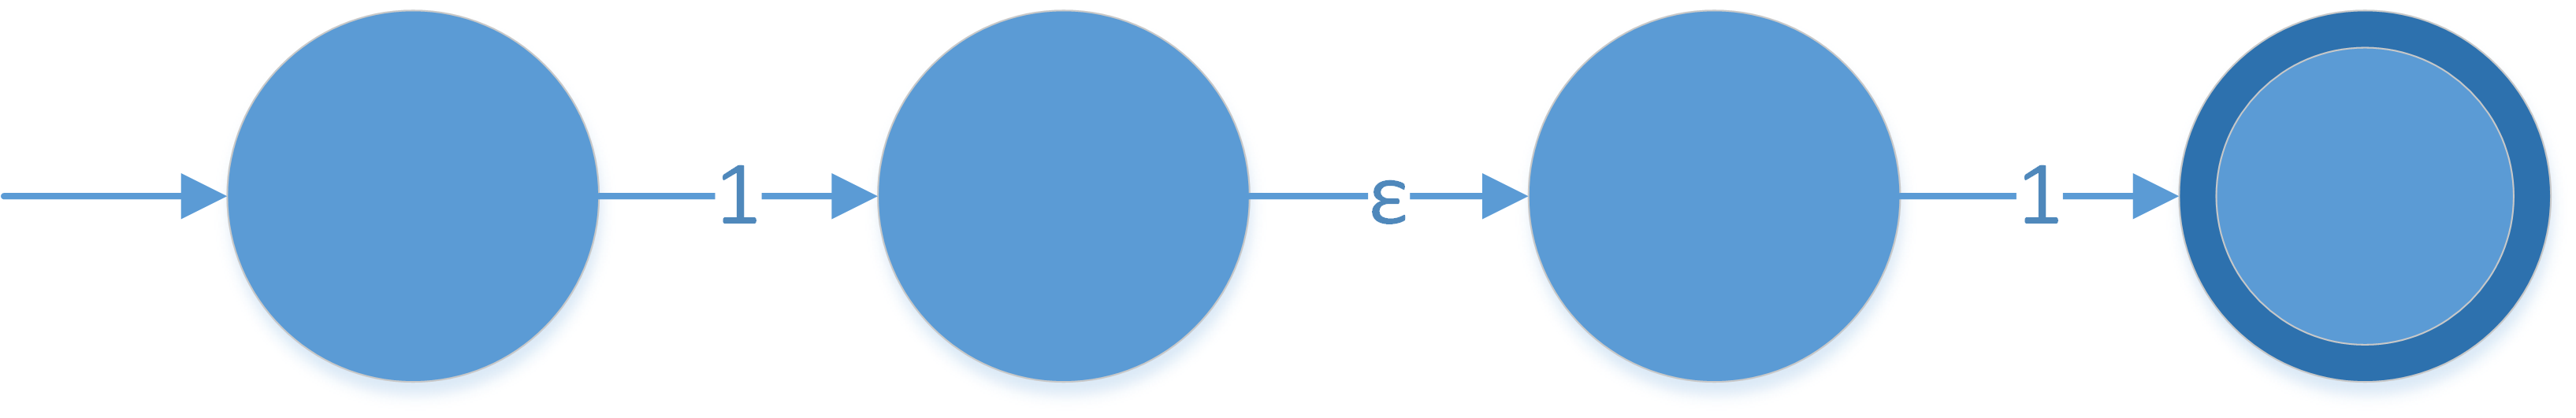
\includegraphics[width=\textwidth]{Fig13x.png}
\label{fig:fig13}
\caption{NFA for $11$}
\end{figure}

Herefter konstrueres NFA'en for $(0\cup1)^*11$ som set på figur \ref{fig:fig14}. Denne NFA kaldes fremover N''.

\begin{figure}[h]%skal placeres rigtigt
\centering
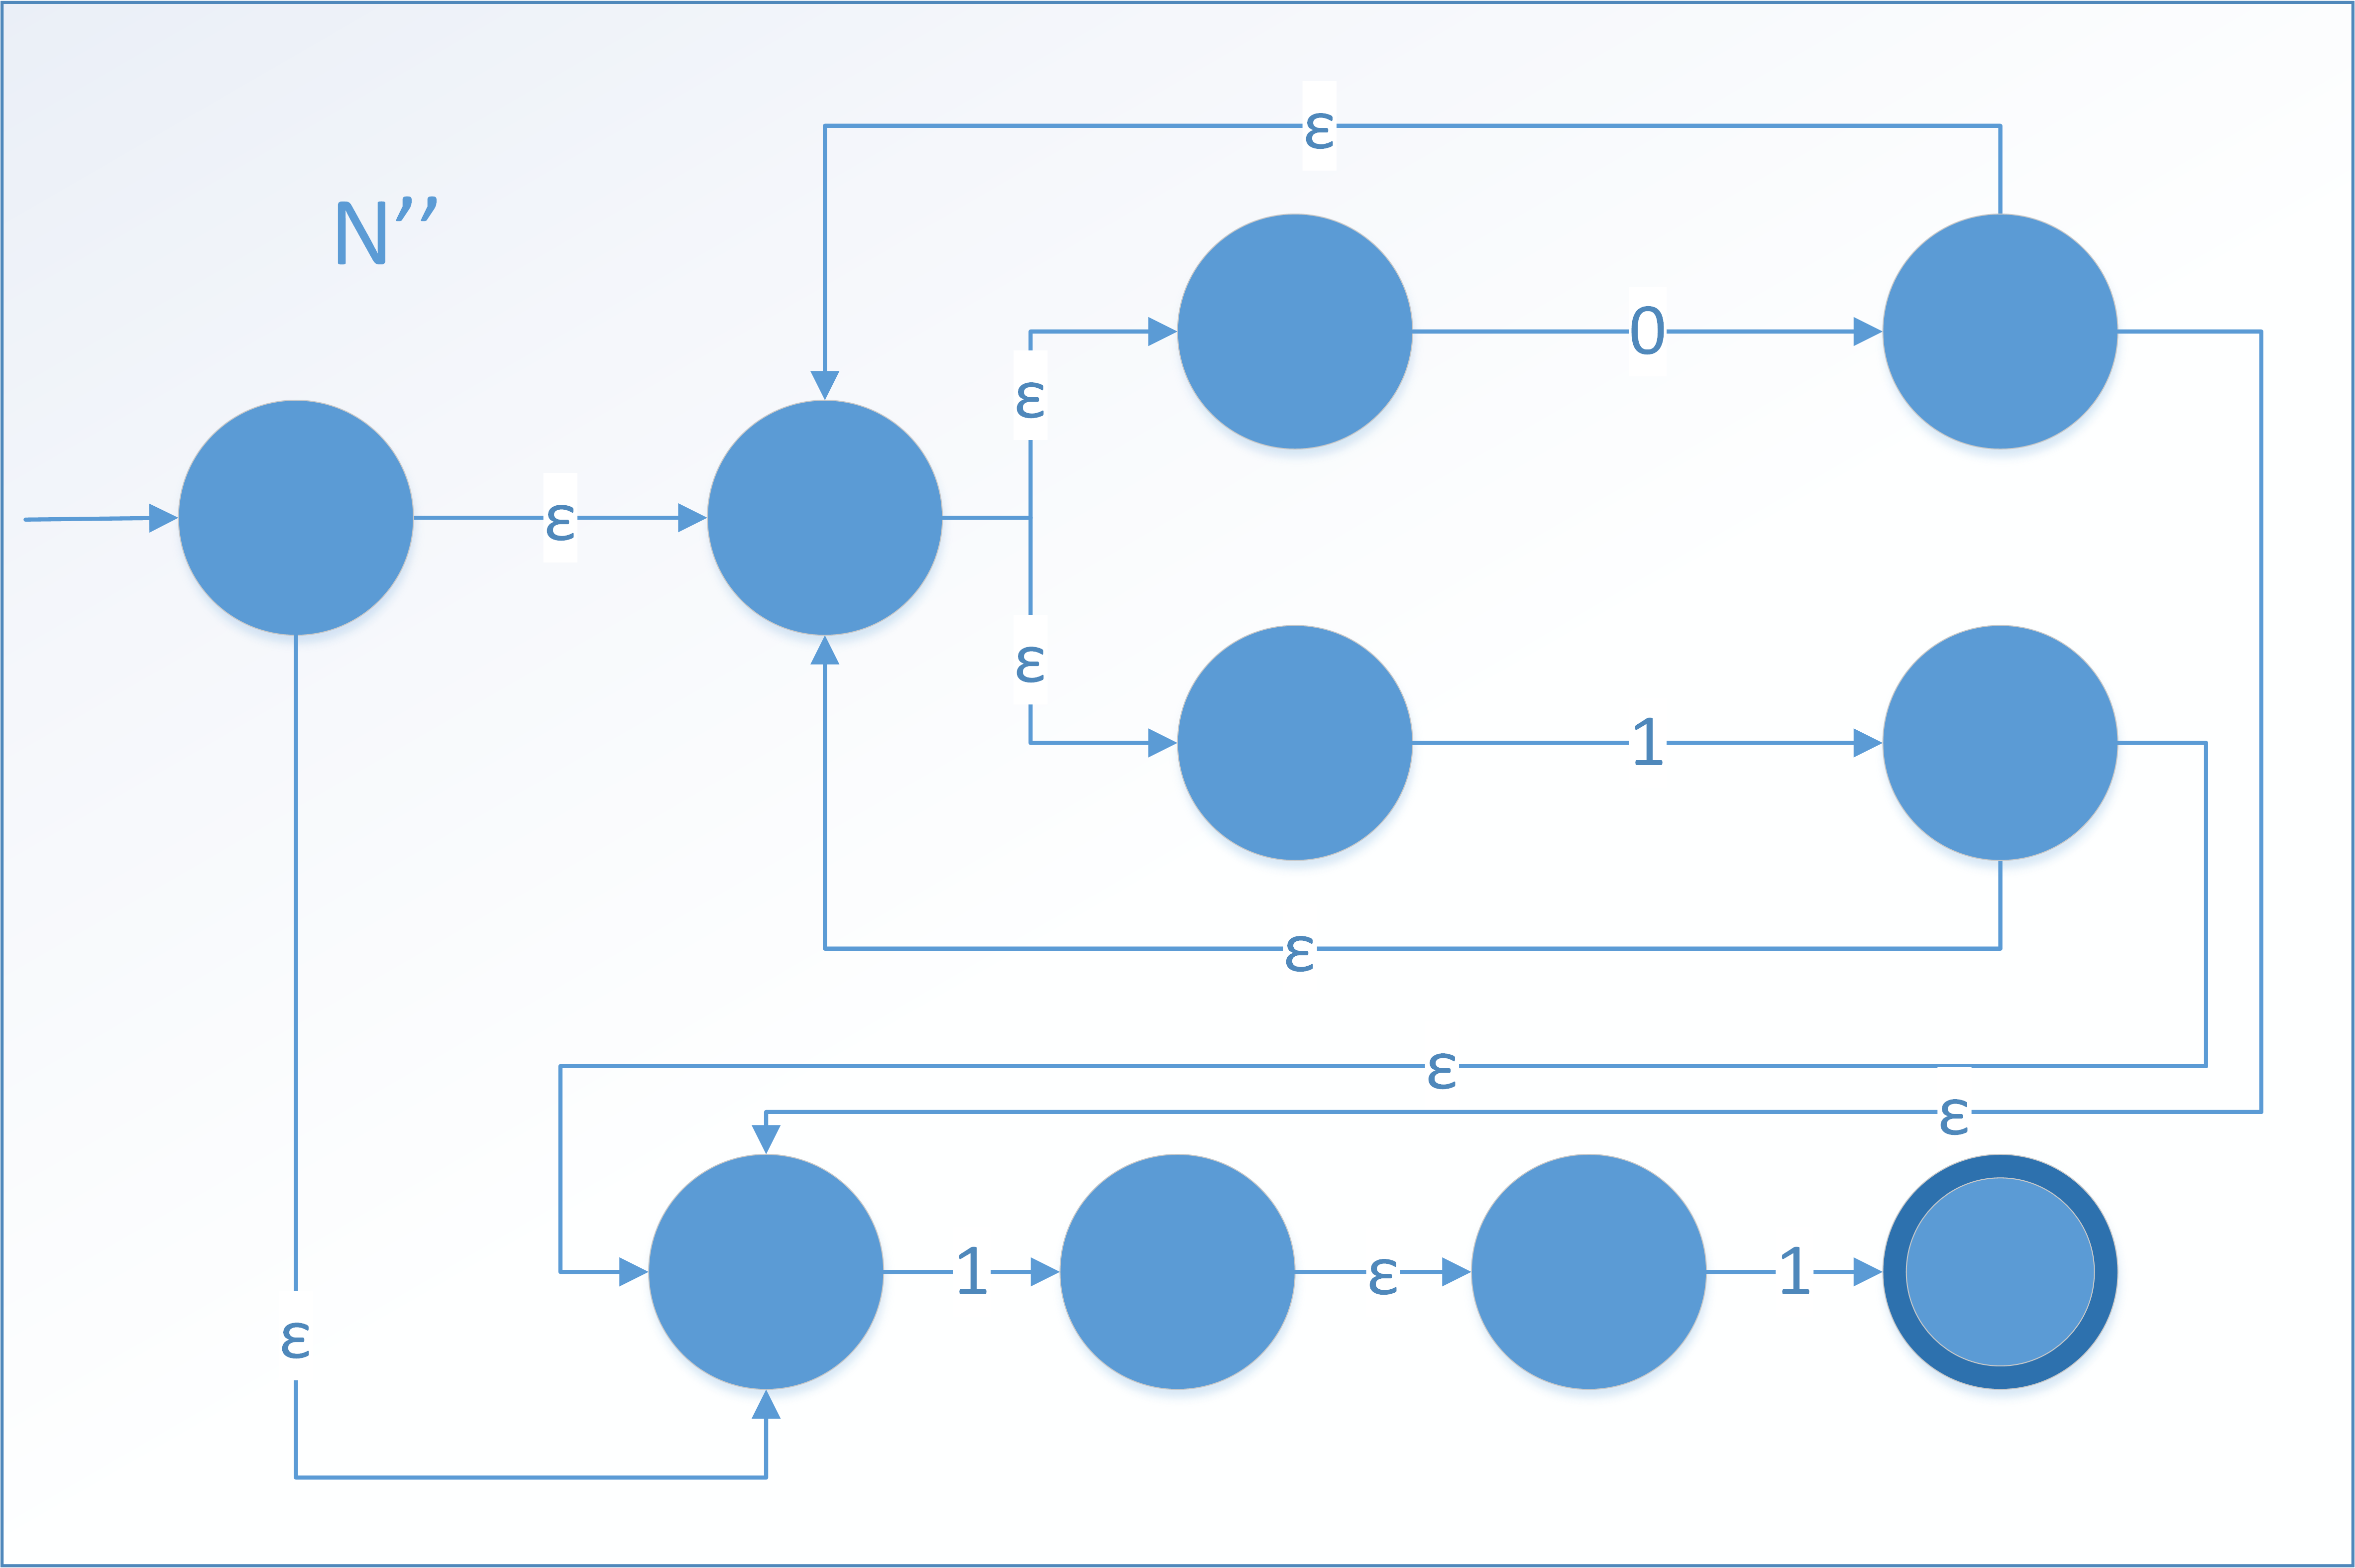
\includegraphics[width=\textwidth]{Fig14x.png}
\label{fig:fig14}
\caption{NFA for $(0\cup1)^*11$}
\end{figure}

Til slut sammensættes N' og N'' som set på figur \ref{fig:fig15}.

\begin{figure}[h]%skal placeres rigtigt
\centering
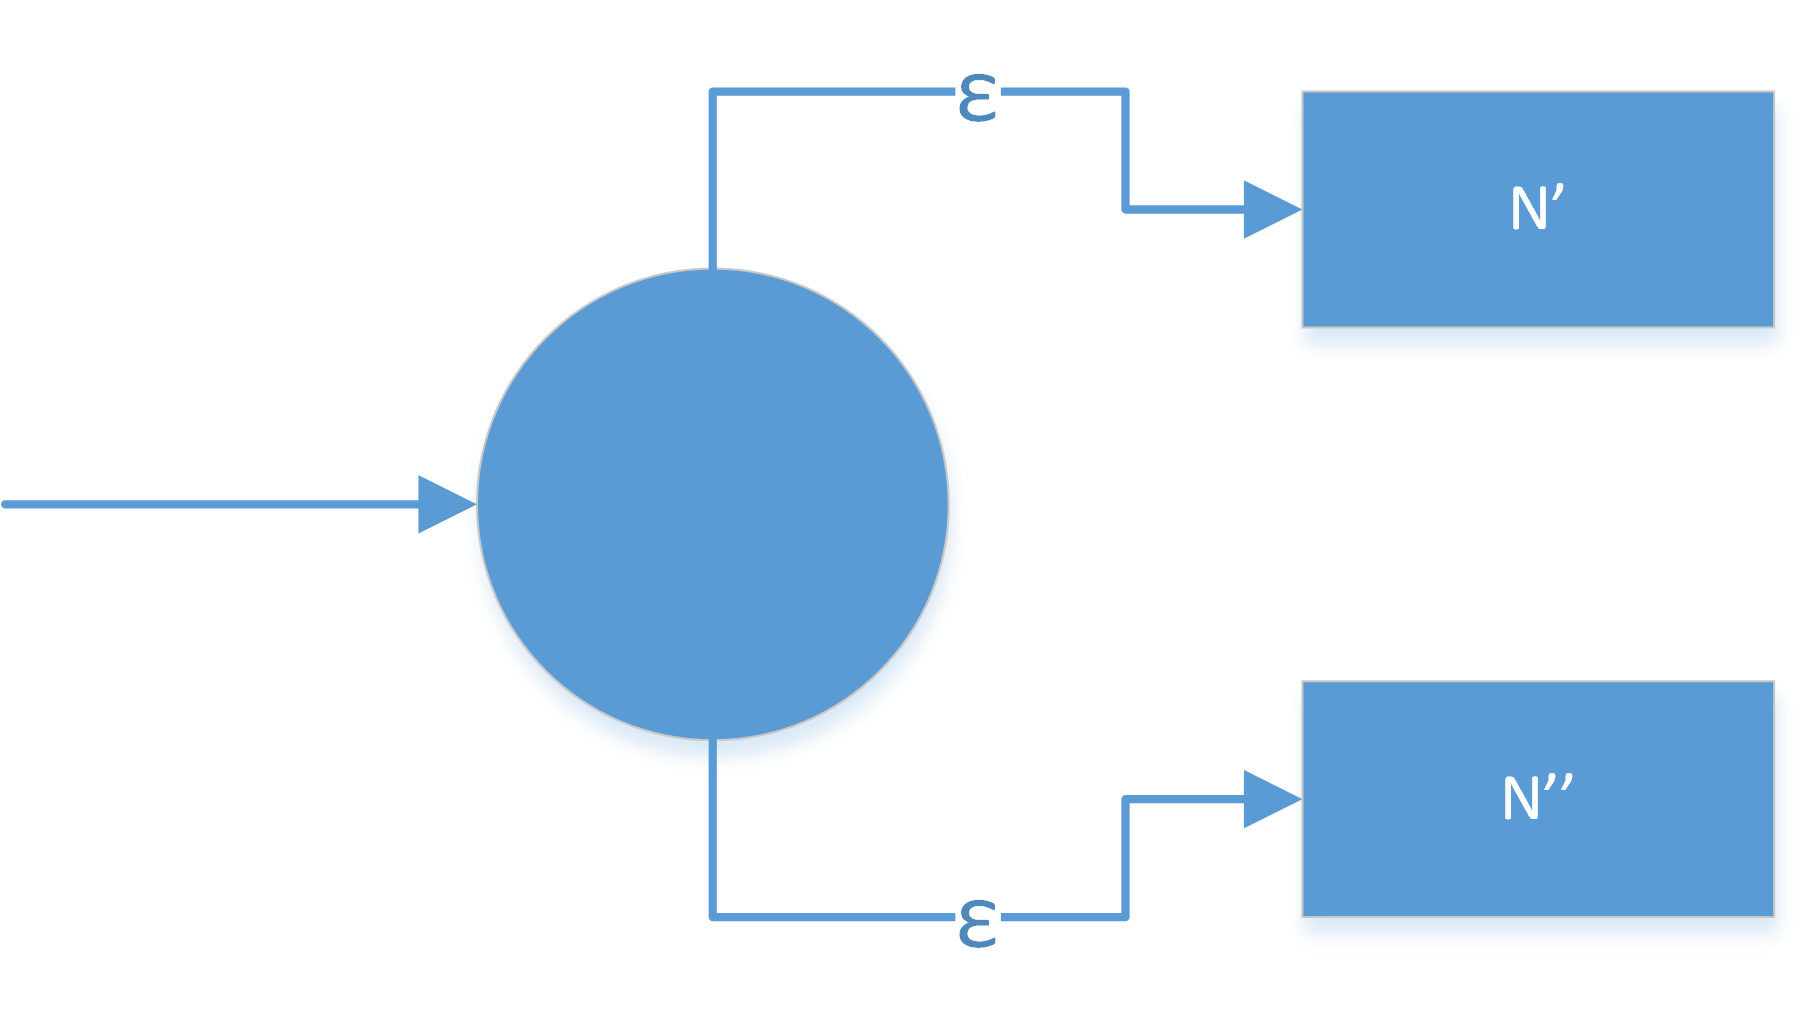
\includegraphics[width=\textwidth]{Fig15x.png}
\label{fig:fig15}
\caption{NFA for $1^*0(1^*01^*01^*)^*  \cup (1 \cup 0)^*11$}
\end{figure}

\chapter{Fra DFA til regulære udtryk}
\section{Teori}
\begin{saetning}For enhver DFA $M$ findes der et regulært udtryk $R$ så $L(R)=L(M)$\end{saetning}
\begin{bevis}
For $M$:
\begin{itemize}
\item Lav $M$ om til en automat med regulære udtryk ved transitionerne, $G_M$.
\item Fjern tilstande fra $G_M$ en ad gangen (men sådan at samme sprog genkendes).
\item Til sidst er der en en start og en sluttilstand, med et regulært udtryk på transitionen fra start til slut.
\end{itemize}

\end{bevis}
\section{GNFA}
\subsection{Teori}
\begin{definition}
En GNFA er en 5-tupel $(Q, \Sigma, q_start, q_accept, \delta)$ hvor der står regulære udtryk på transitionerne (se figur \ref{fig:fig16}).
\end{definition}
\begin{figure}[h]%skal placeres rigtigt
\centering
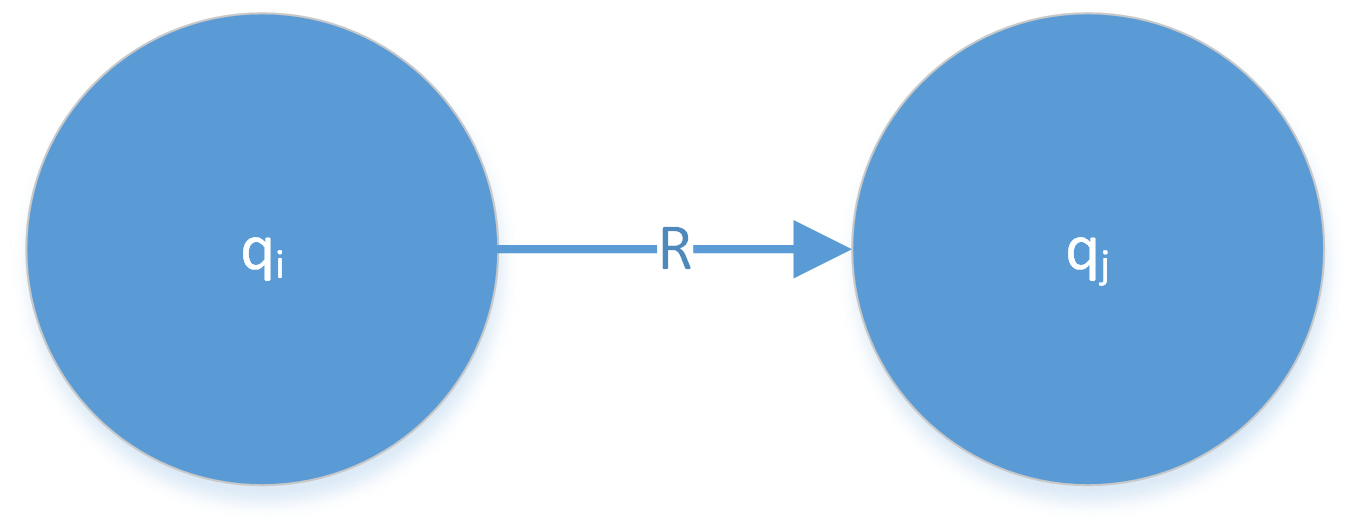
\includegraphics[width=\textwidth]{Fig16x.png}
\label{fig:fig16}
\caption{En GNFA med regulære udtryk på transitionerne}
\end{figure}
dvs.

$\delta: Q\setminus\{q_{accept}\}\times Q\setminus\{q_{start}\} \Ra \mathcal{R}$
hvor $\mathcal{R}$ betegner mængden af regulære udtryk.

En GNFA overholder denne bordskik:
\begin{enumerate}
\item En transition mellem hvert par af tilstande
\item Ingen transitioner \underline{fra} $q_{accept}$
\item Ingen transitioner \underline{til} $q_{start}$
\end{enumerate}
En GNFA accepterer en streng $w$ hvis 

$w = S_1 \dots S_n$

og der er en følge af tilstande $r_1 \dots r_n$ så:
\begin{itemize}
\item $r_1 = q_{start}$
\item For alle $r_i (1 \leq i < n)$ gælder $\delta (r_i, r_{i+1})=R_i$ og $S_i \in L(R_i)$
\item $r_n = q_{accept}$
\end{itemize}

\subsection{eksempel på en GNFA}
På figur \ref{fig:fig17} ses et eksempel på en GNFA. Her accepteres fx strengen "aaba". Dette kan vises ved at "aaba" kan deles op i $\epsilon$ a a b a $\epsilon$
\begin{figure}[h]%skal placeres rigtigt
\centering
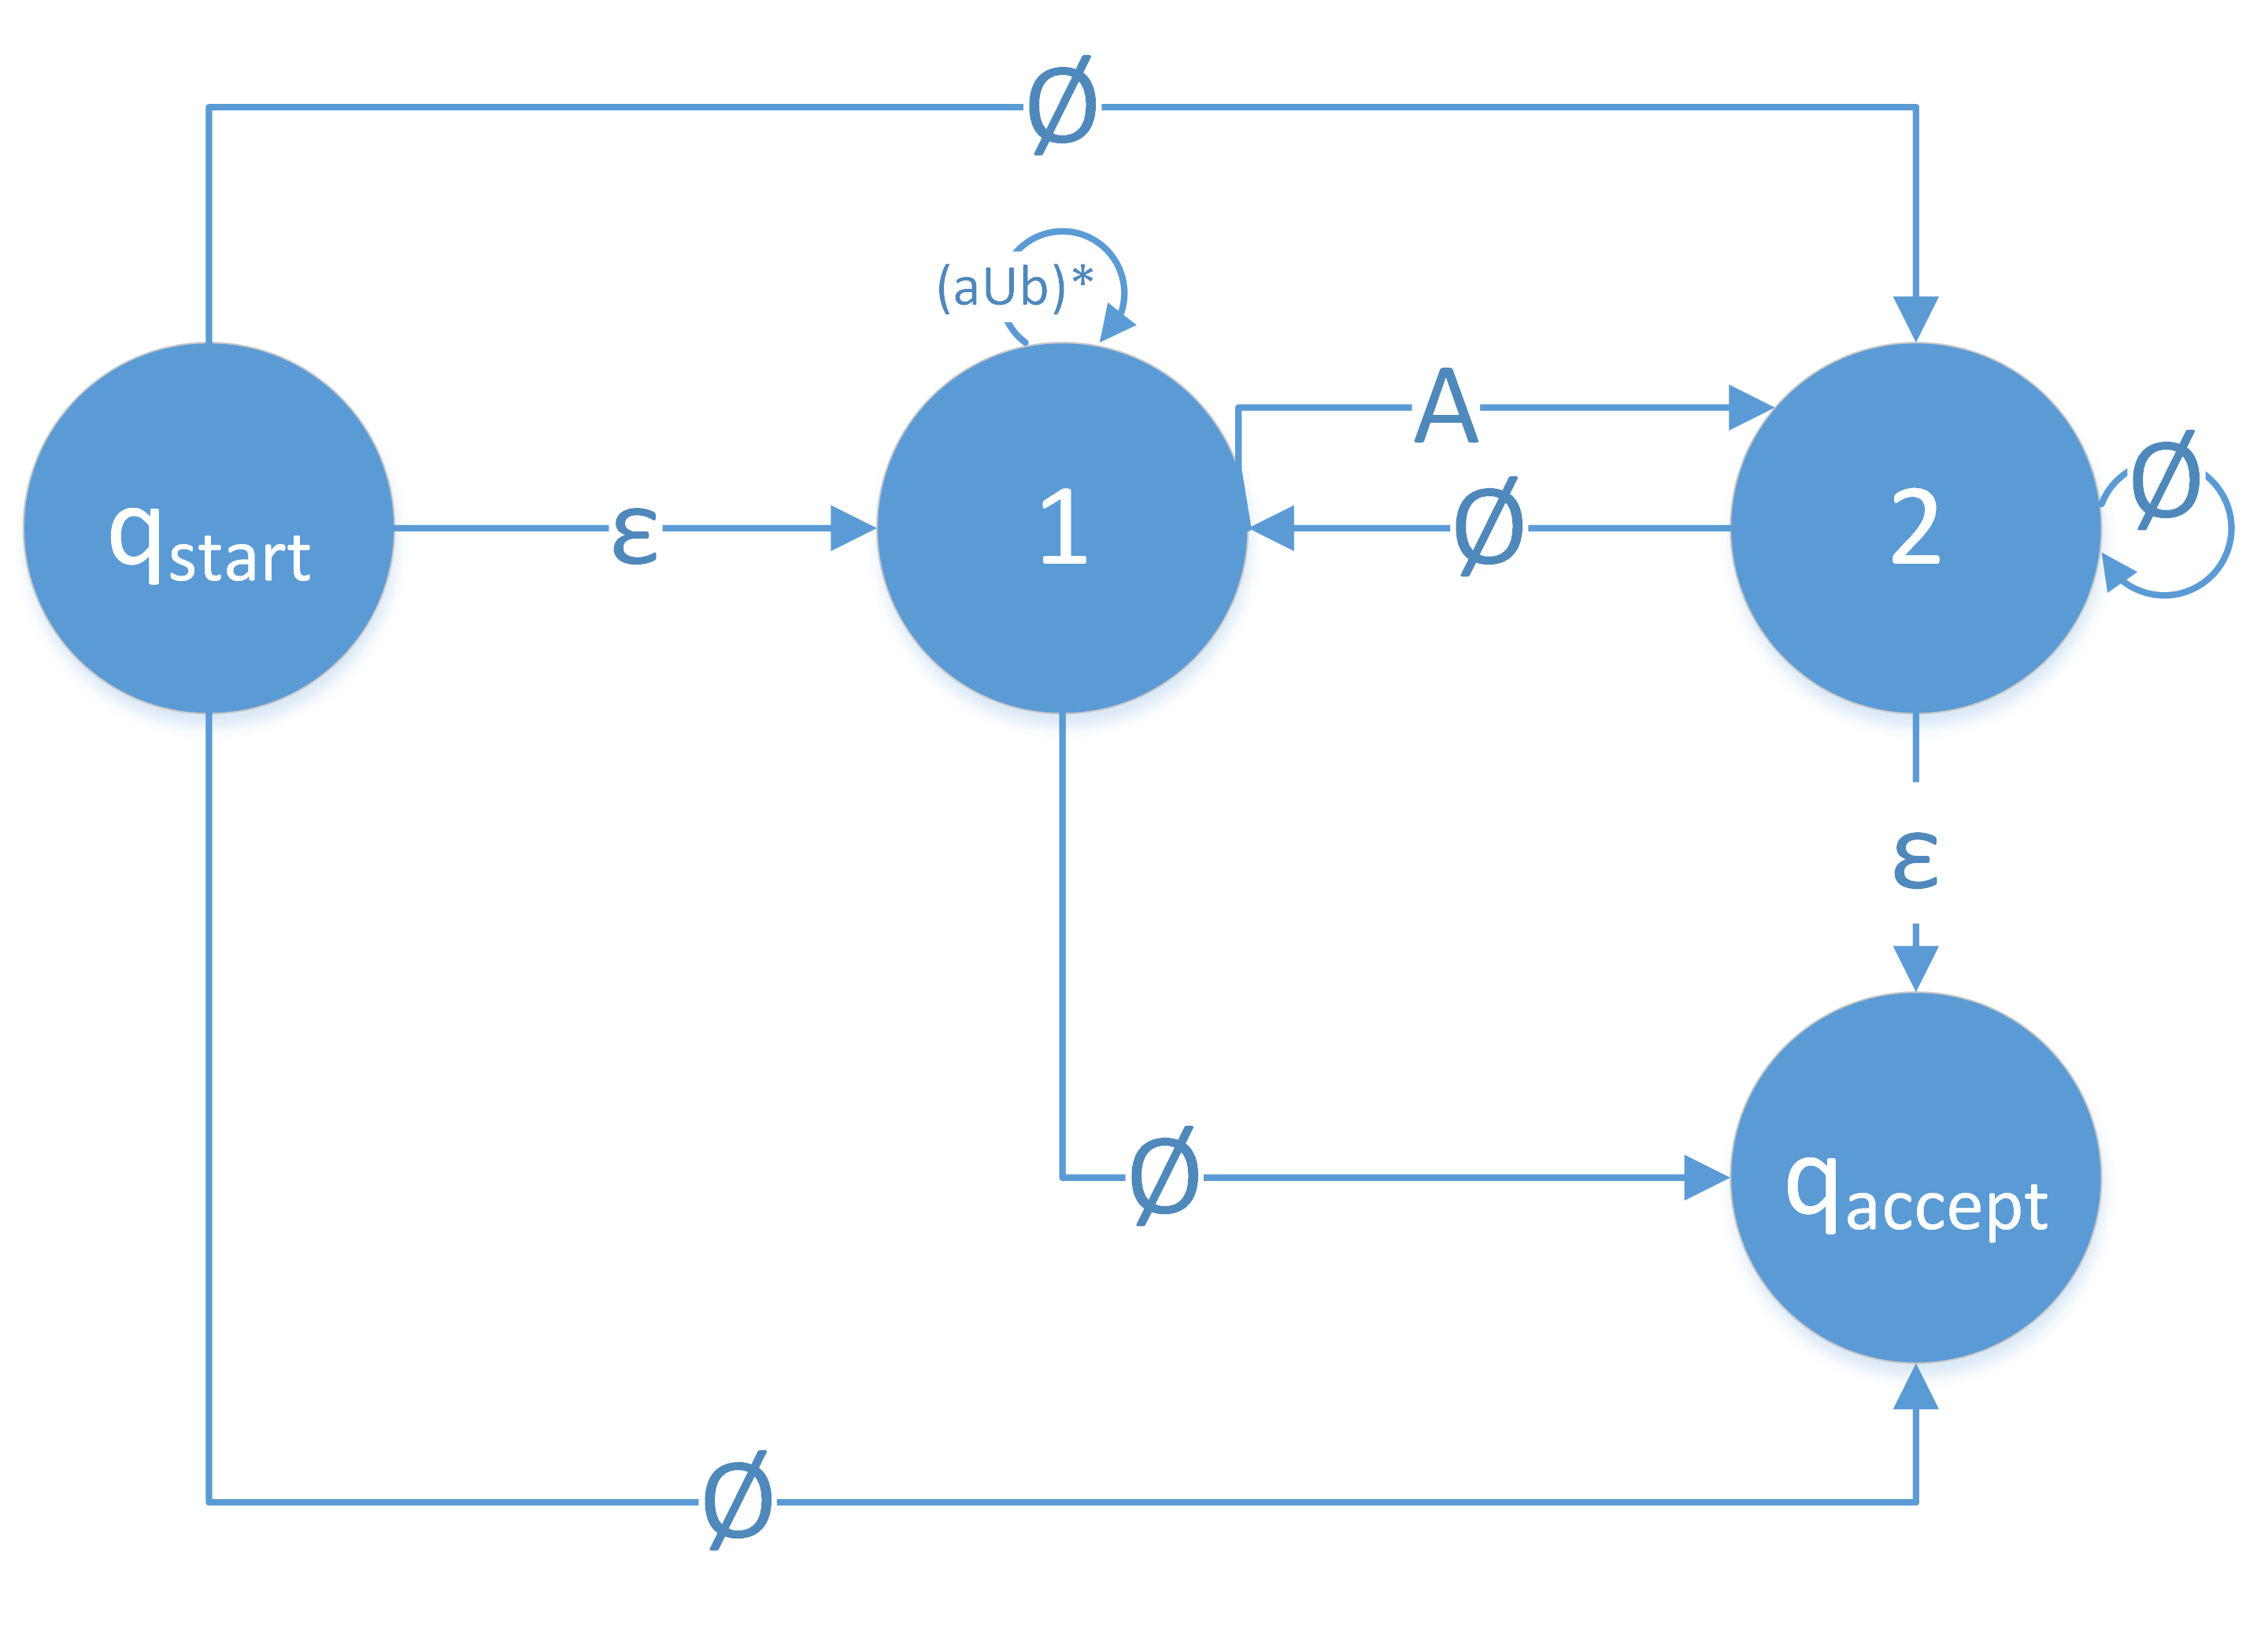
\includegraphics[width=\textwidth]{Fig17x.png}
\label{fig:fig17}
\caption{Et eksempel på en GNFA}
\end{figure}

Her accepteres fx strengen "aaba". Dette kan vises ved at "aaba" kan deles op i $\epsilon$ a a b a $\epsilon$, se figur \ref{fig:fig18}.

\begin{figure}[h]%skal placeres rigtigt
\centering
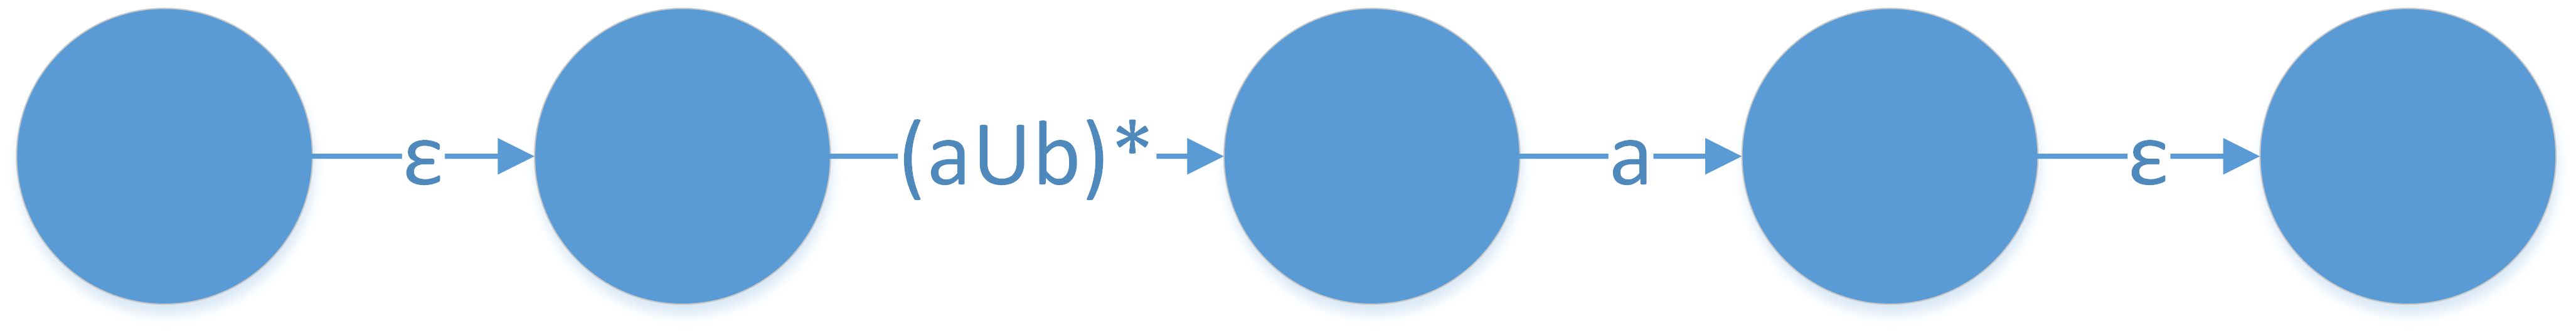
\includegraphics[width=\textwidth]{Fig18x.png}
\label{fig:fig18}
\caption{En gennemgang af "aaba" ved GNFA'en fra figur \ref{fig:fig17}}
\end{figure}

\subsection{Fra DFA til regulære udtryk}
Givet en DFA $M$ der ønsket skrevet i form at regulære udtryk.
Først skal $M$ laves om til en GNFA.
Dette gøres ved:
\begin{itemize}
\item Indfør ny $q_{start}$ og en transition $\epsilon$ til det gamle startpunkt ved $M$
\item Indfør ny $q_{accept}$ og lav for hver gammen accepttilstand en $\epsilon$ transition til $q_{accept}$
\item Hvis der ikke er en transition mellem $q_i$ og $q_j$ i M tilføjes en transition mærket $\emptyset$
\item Saml transitioner med $\cup$ så en transition mærket "a,b" i stedet bliver mærket $a\cup b$
\end{itemize}

Herefter fjernes tilstandene en efter en, så der kun er $q_{start}$ og $q_{accept}$ tilbage.
For at fjerne en tilstand så sproget bevares vælges en $q_{rip}$ som skal fjernes, hvorom det gælder at $q_{rip} \neq q_{start}$ og $q_{rip} \neq q_{accept}$. For alle andre tilstande ved vi pga. bordskik i forhold til GNFA hvordan man kan fjerne $q_rip$ og erstatte transitionen med et regulært udtryk. Dette kan ses på figur \ref{fig:fig19}.

\begin{figure}[h]%skal placeres rigtigt
\centering
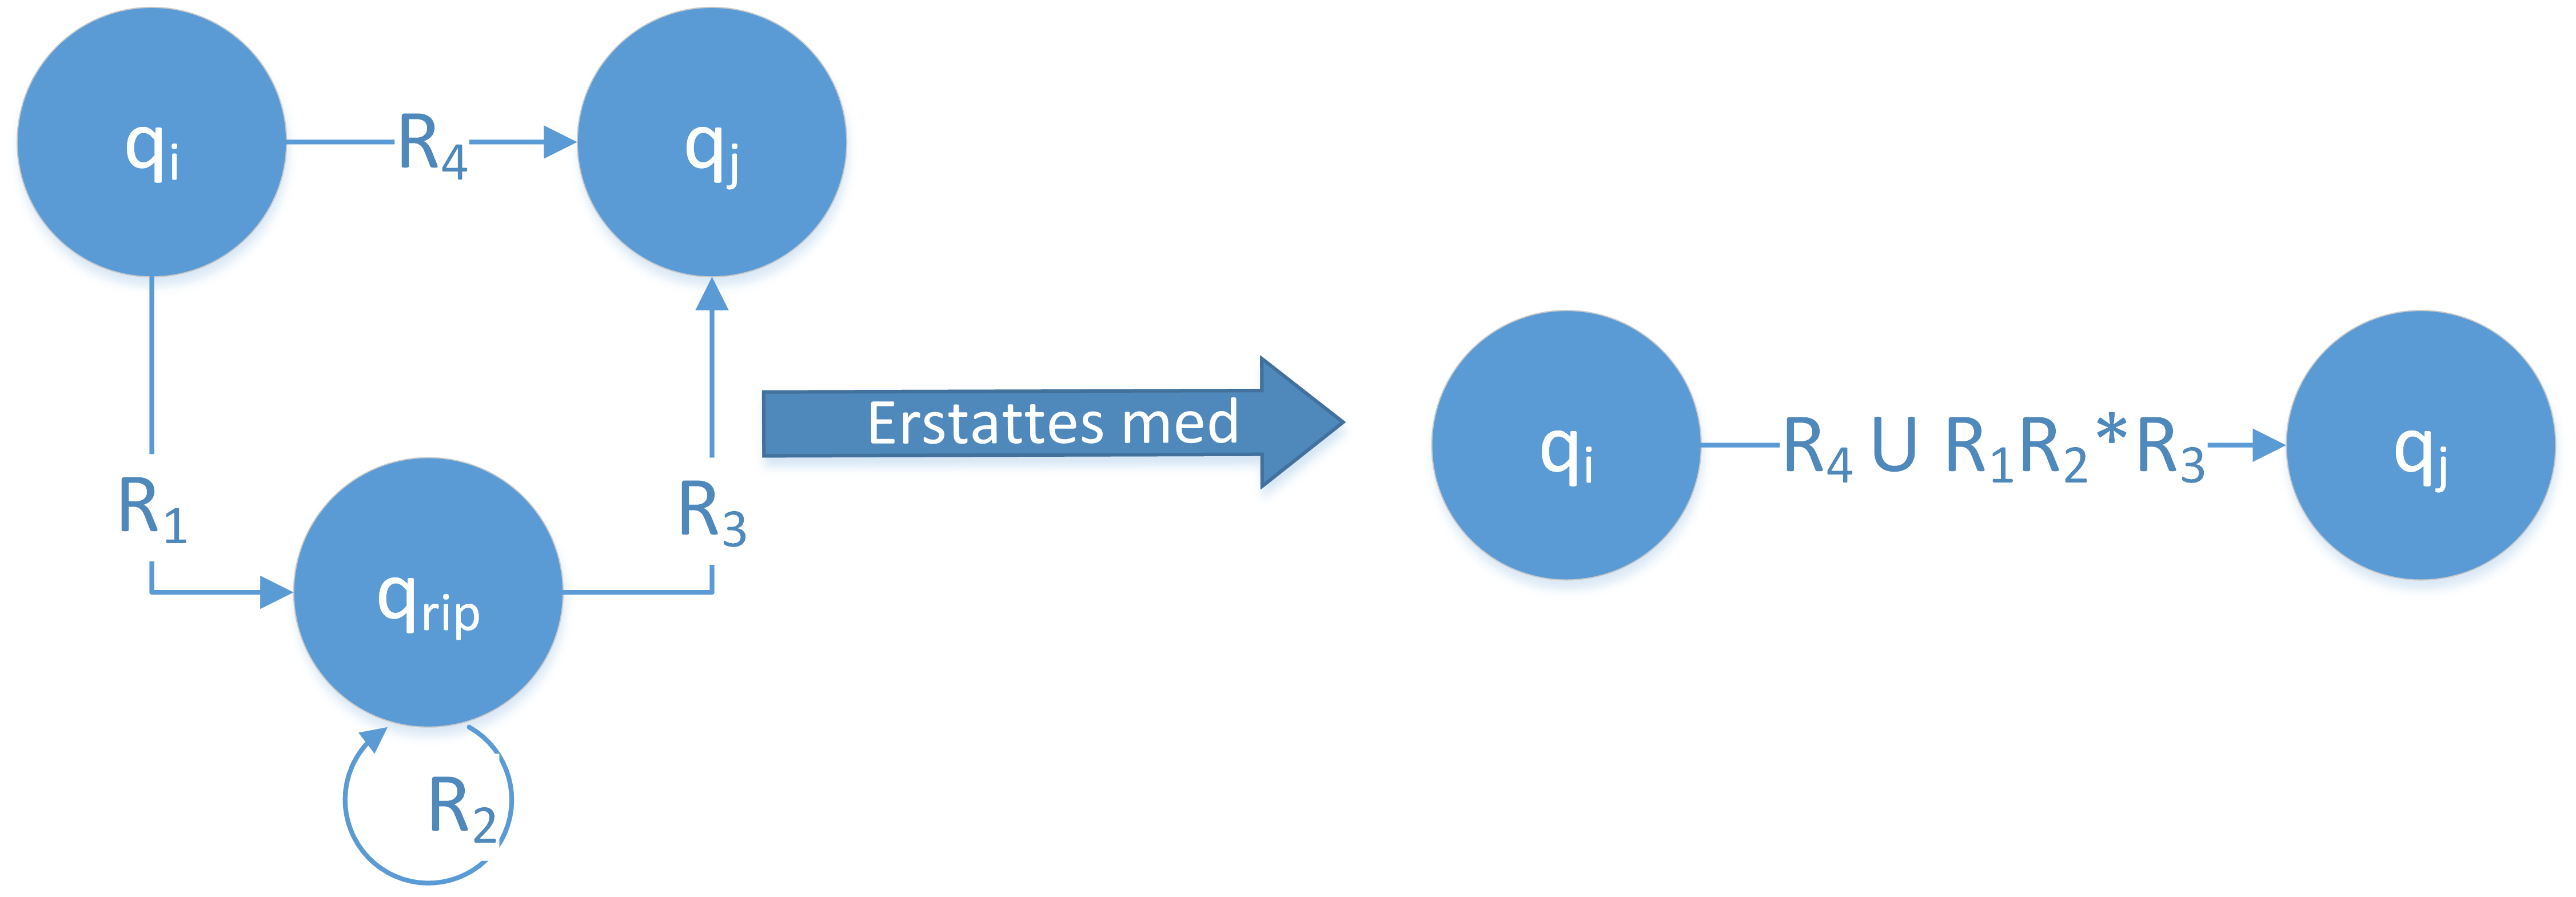
\includegraphics[width=\textwidth]{Fig19x.png}
\label{fig:fig19}
\caption{Metode til at fjerne en tilstand fra en GNFA}
\end{figure}

\subsection{Eksempel}
Givet er en DFA kaldet $m$, som kan ses på figur \ref{fig:fig20}.
\begin{figure}[h]%skal placeres rigtigt
\centering
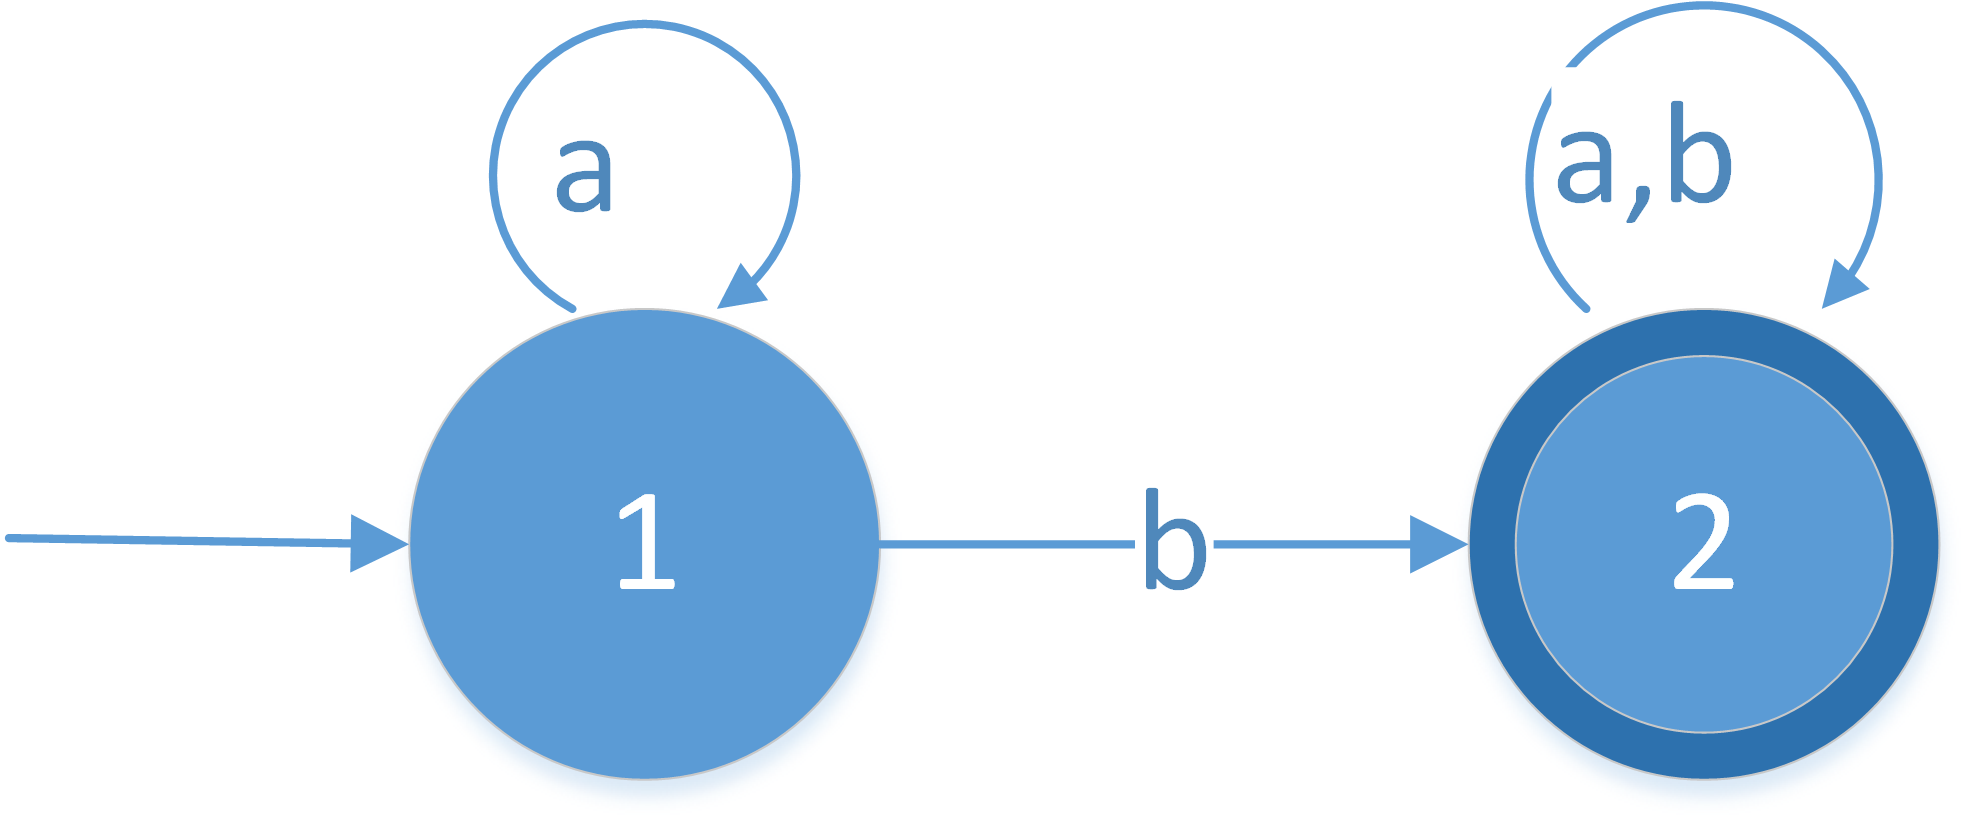
\includegraphics[width=\textwidth]{Fig20x.png}
\label{fig:fig20}
\caption{En DFA $M$}
\end{figure}

Herefter laves en GNFA ud fra DFA'en $M$, som kan ses på figur \ref{fig:fig21}.
\begin{figure}[h]%skal placeres rigtigt
\centering
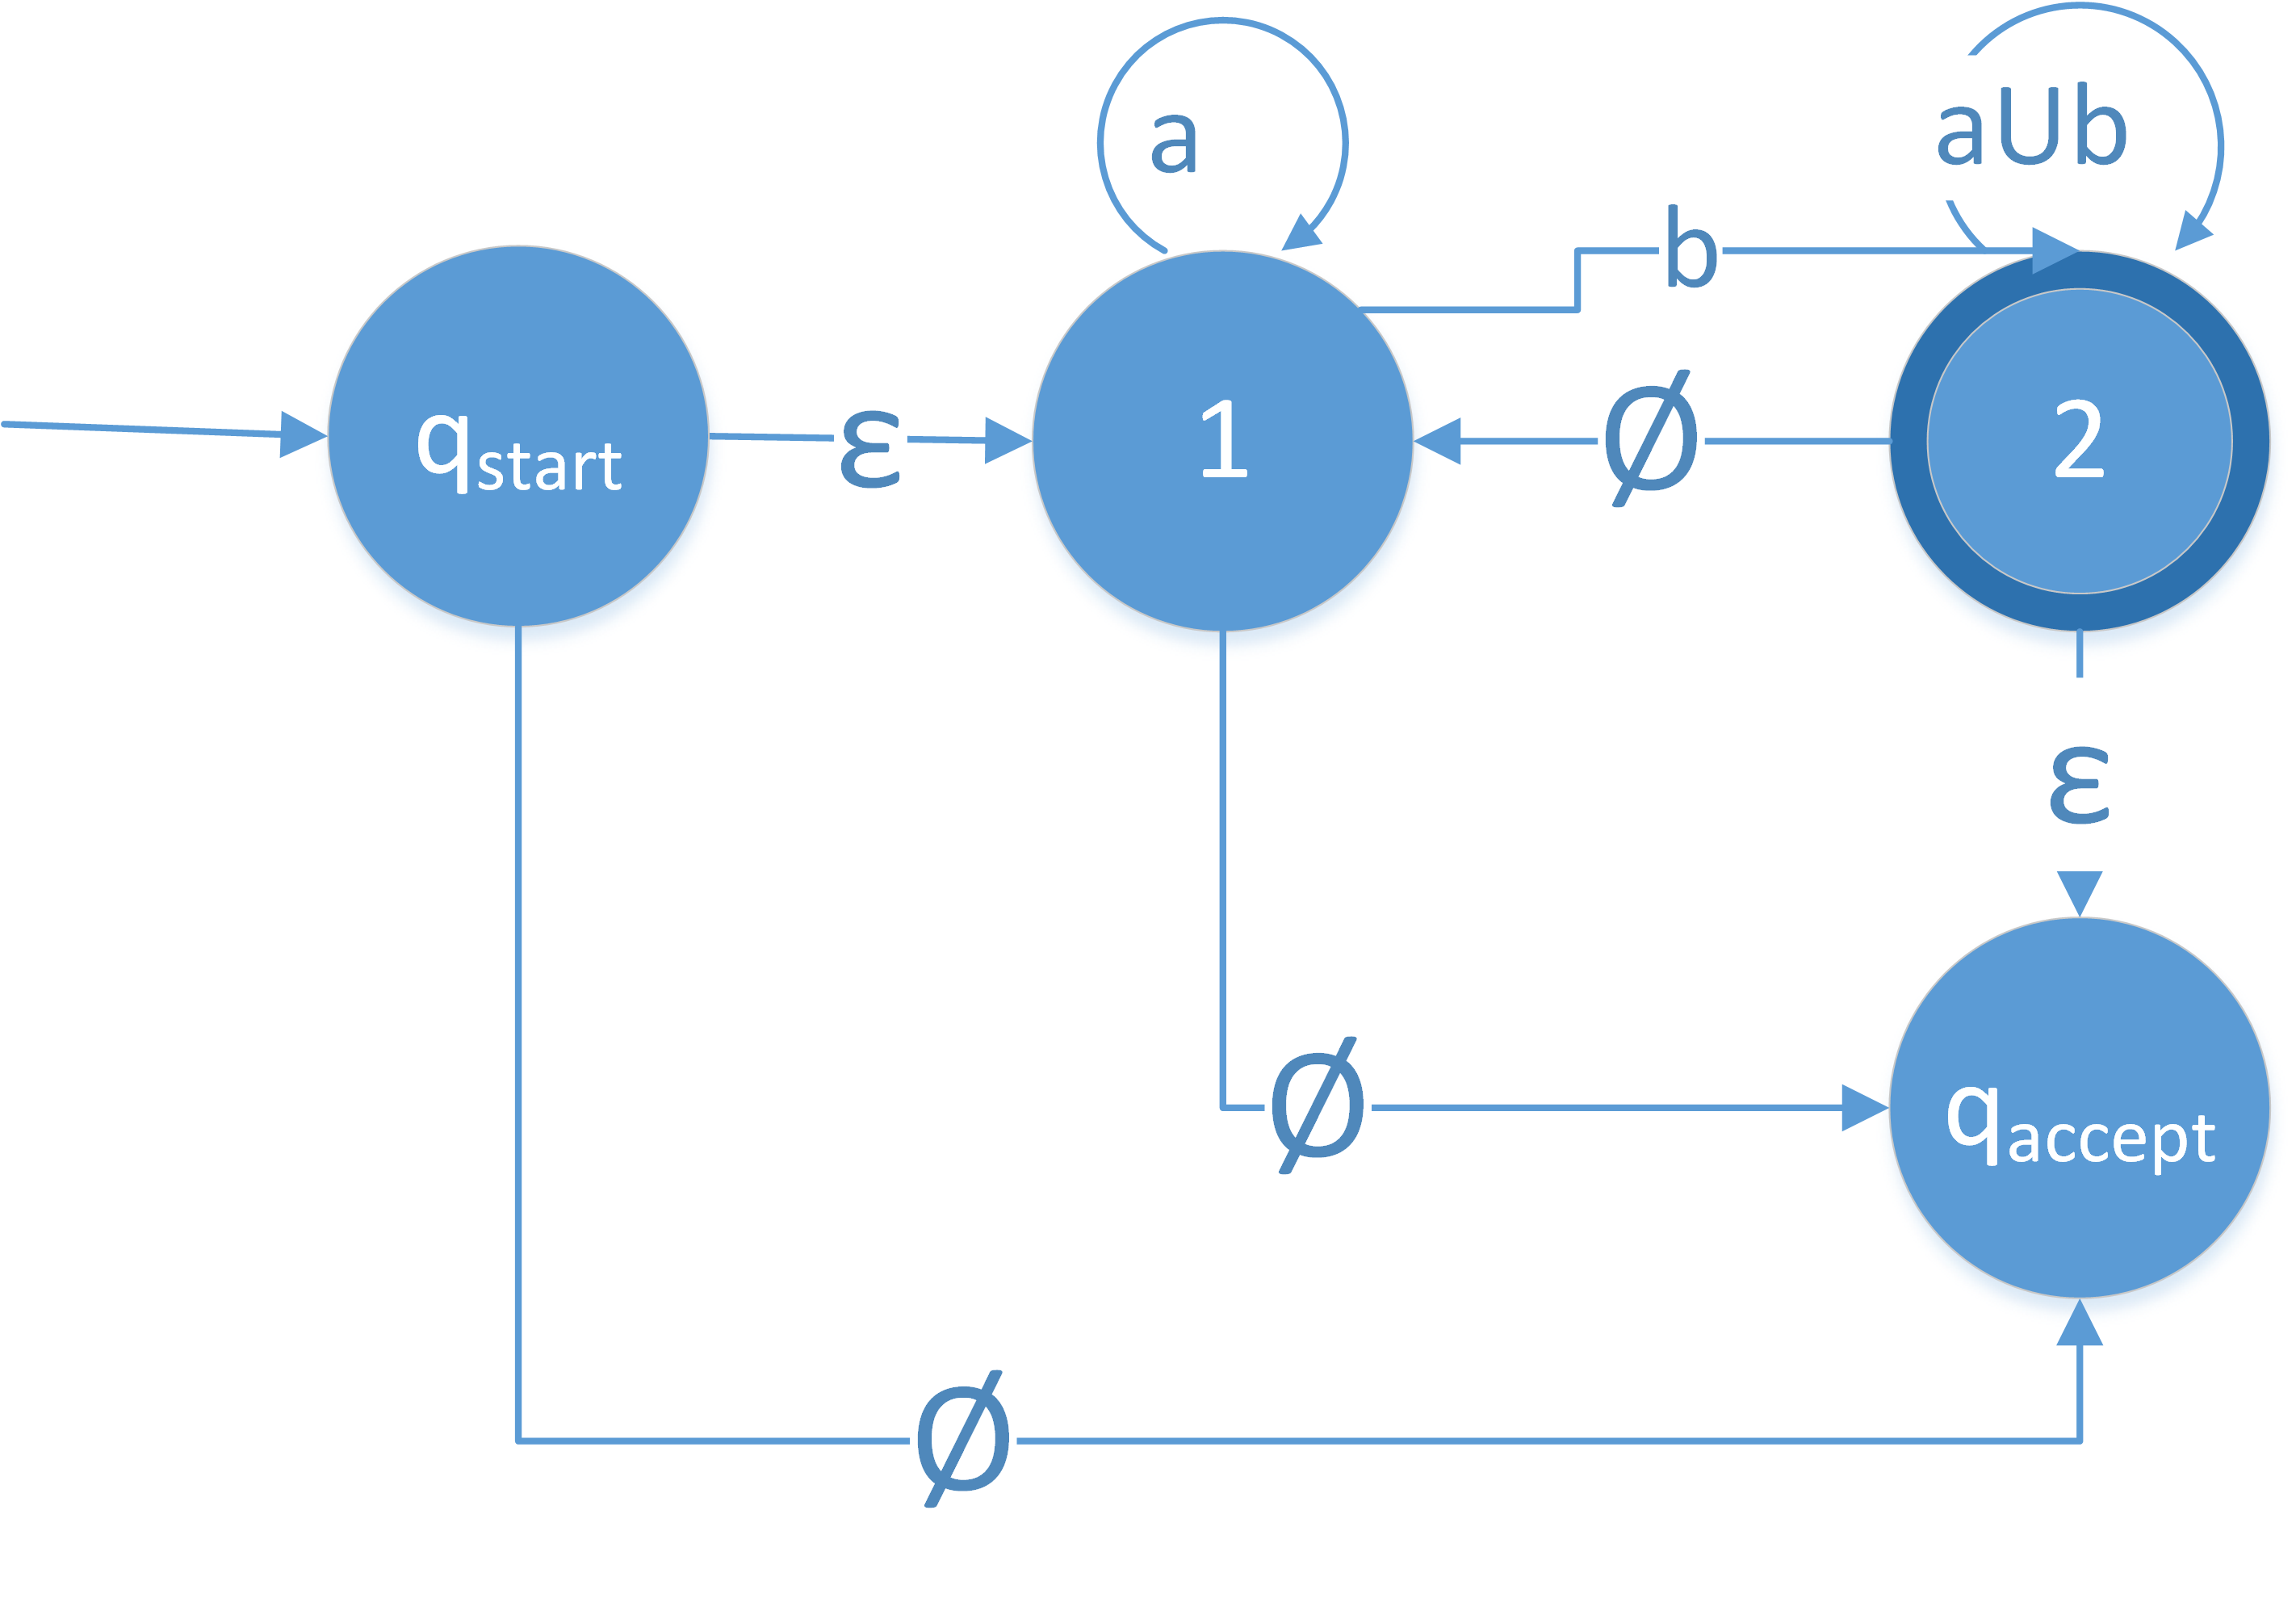
\includegraphics[width=\textwidth]{Fig21x.png}
\label{fig:fig21}
\caption{En GNFA ud fra DFA'en $M$}
\end{figure}

Herefter sættes tilstand 1 som $q_{rip}$ som ses på \ref{fig:fig22}.
\begin{figure}[h]%skal placeres rigtigt
\centering
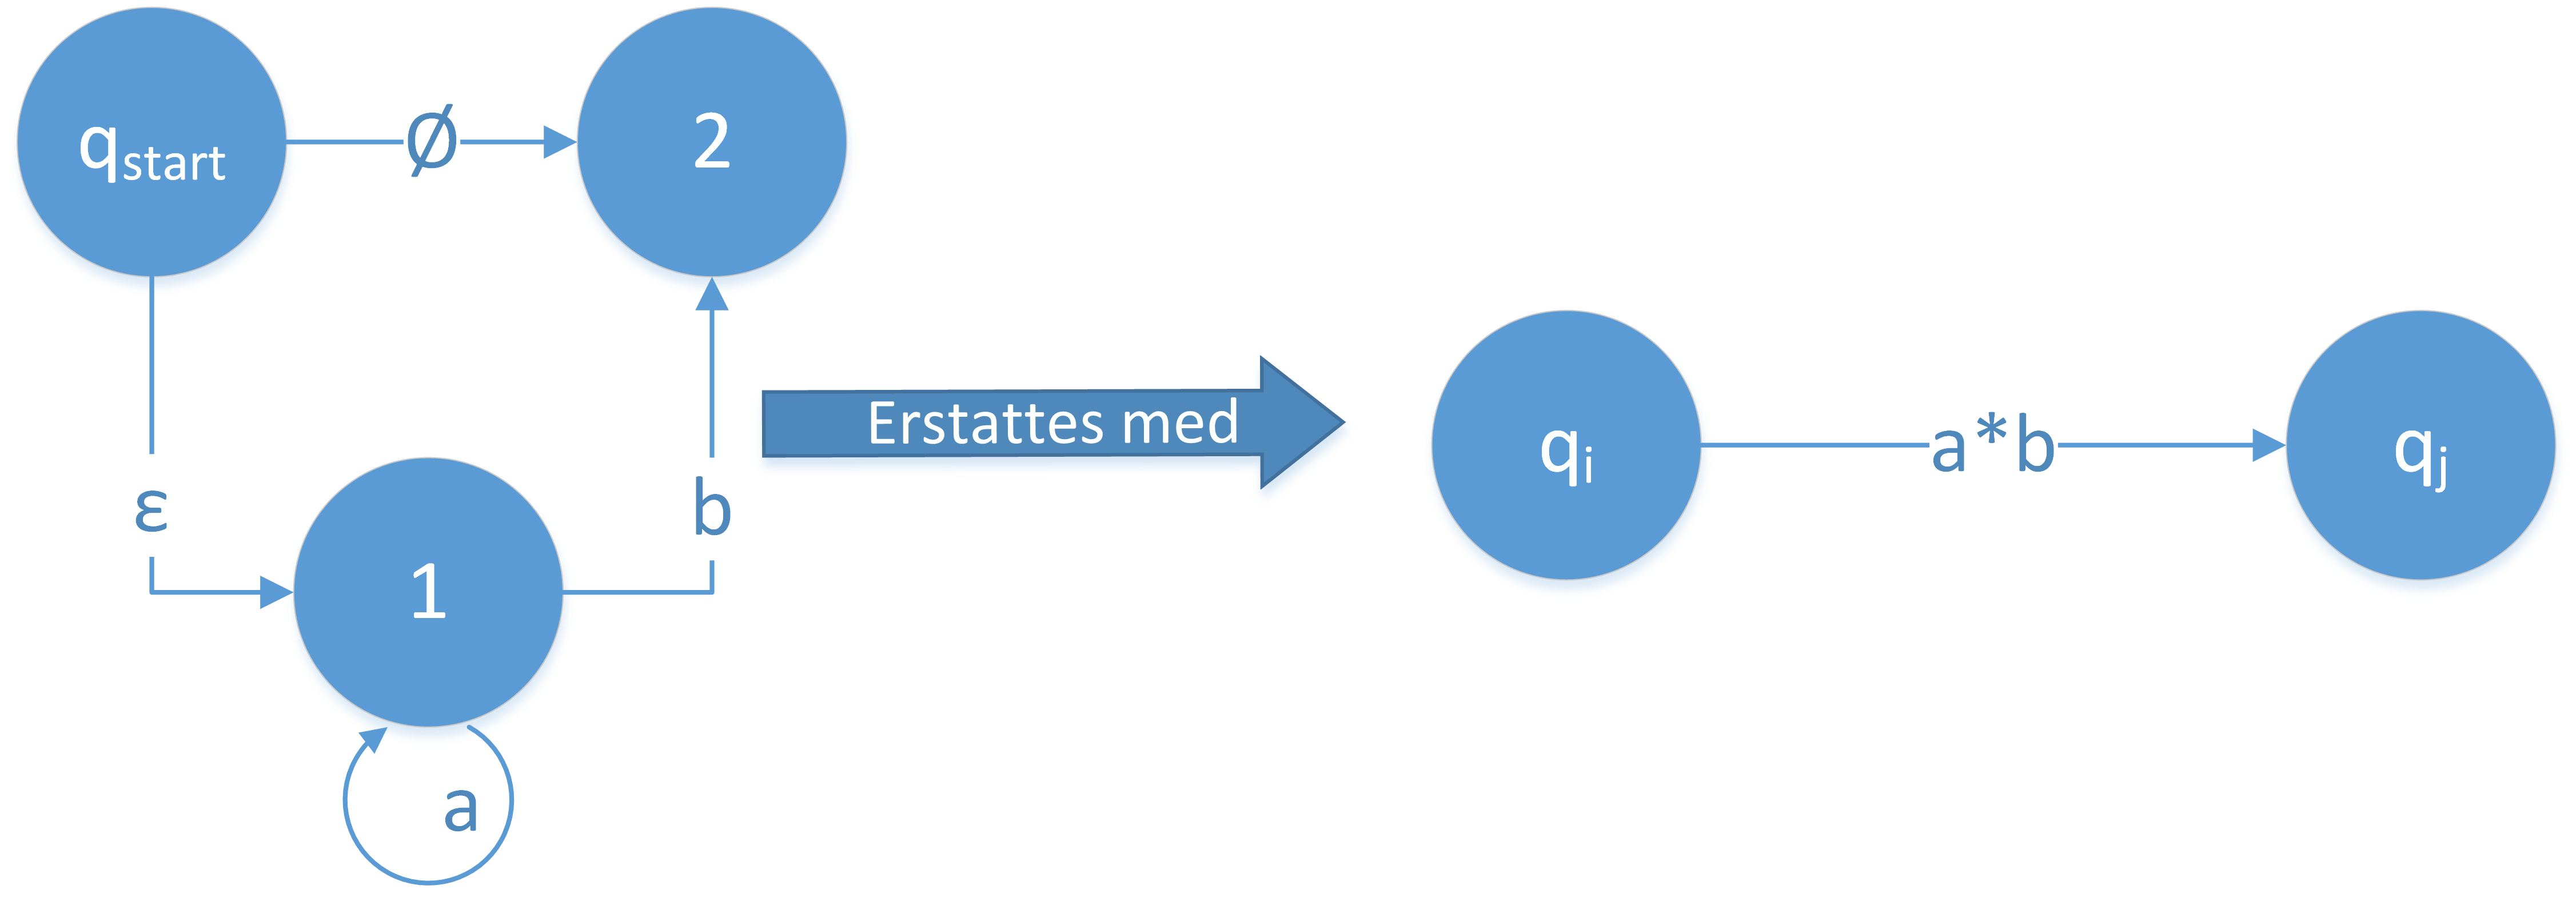
\includegraphics[width=\textwidth]{Fig22x.png}
\label{fig:fig22}
\caption{Udledningen af det regulære udtryk der skal erstatte tilstand 1}
\end{figure}
Det samme gøres, hvor tilstand 2 bliver sat som $q_{rip}$ og slutresultatet bliver det regulære udtryk $a^*b(a\cup b)^*$.
\chapter{Gyser}
\section{Termolig}
\begin{itemize}
\item Regulære udtryk \underline{beskriver} sprog, automater \underline{genkender} sprog.
\begin{itemize}
\item ikke "regulære udtryk genkender"
\item ikke "regulære udtryk accepterer"
\end{itemize}
\end{itemize}
\section{Ingen Ad-Hoc-løsninger}
\begin{itemize}
\item Brug algoritmen!
\item Lad være med at gætte $\Ra$ det er som regel forkert!
\end{itemize}
\section{Ingen smarte genveje}
Gør det rigtigt fra starten, og undgå smarte genveje. Se figur \ref{fig:fig23}.
\begin{figure}[h]%skal placeres rigtigt
\centering
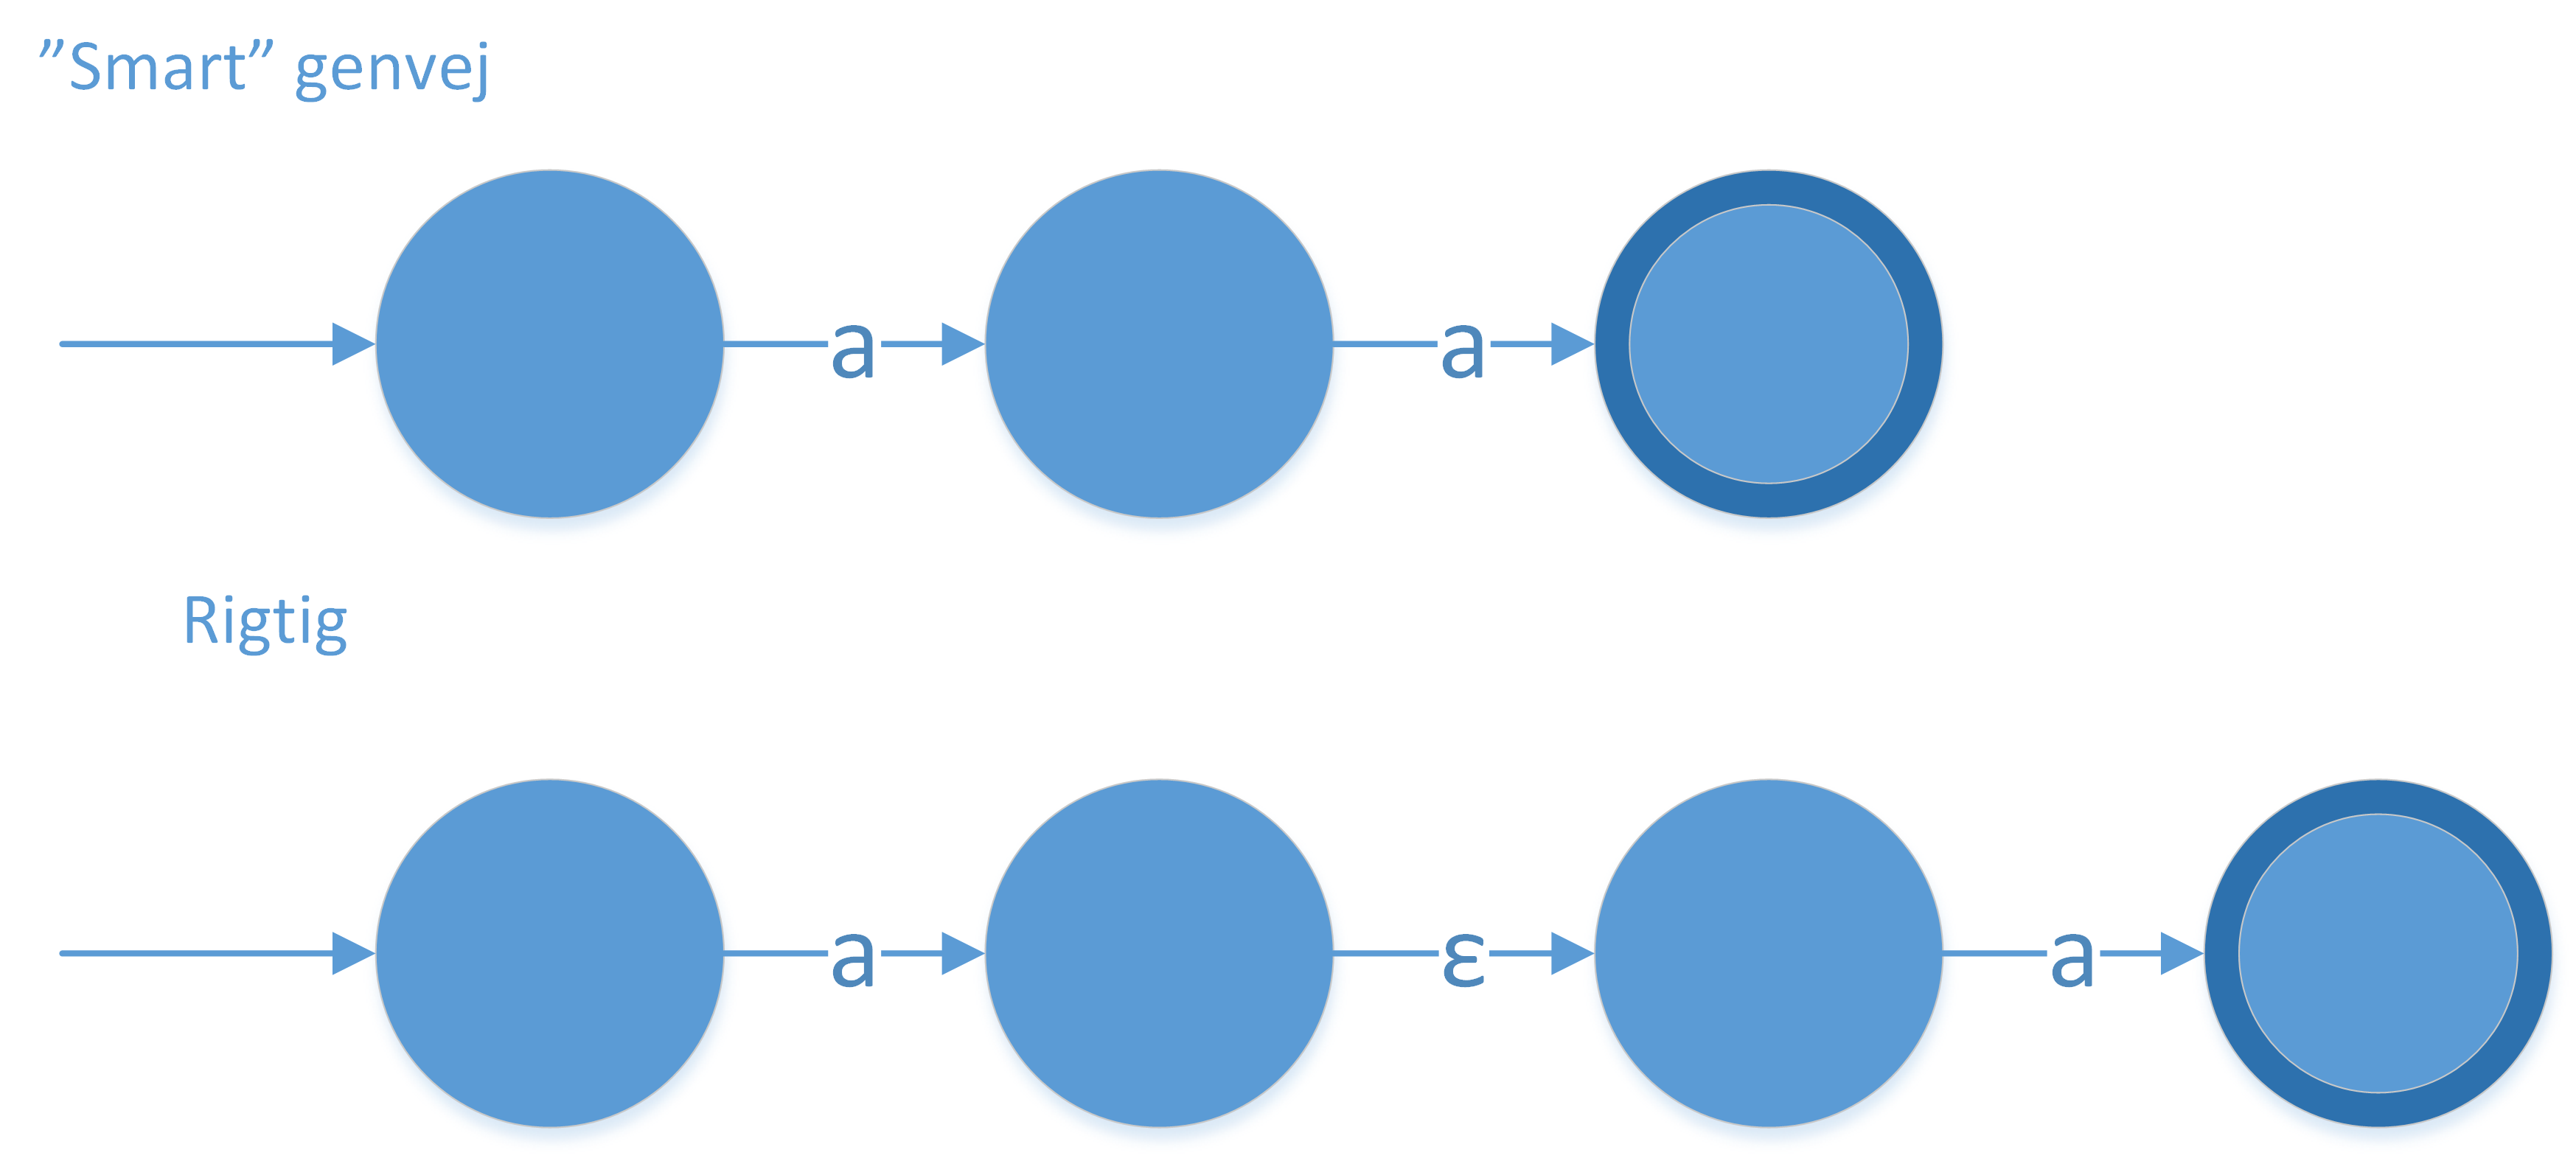
\includegraphics[width=\textwidth]{Fig23x.png}
\label{fig:fig23}
\caption{Undgå smarte genveje}
\end{figure}
\end{document}
